\chapter{Signal Modeling} \label{chapter:signal}

\section{Building a Hypothesis}

    The core of the scientific method is in the practice of making a hypothesis
        and of then testing that hypothesis through experiment.
    The hypothesis made in this analysis is that the Standard Model of Particle Physics is mostly correct
        and that deviations from this theory should manifest in the probabilities of physical processes.
    I have spent the past several chapters discussing the experimentation process.
    Now it is time to discuss how I constructed a hypothesis that can be tested against the data provided from that experiment.

    The most basic hypothesis made in this analysis is that the di-Higgs process exists at all.
    Unfortunately, a direct measurement of the di-Higgs process is unlikely to occur in this study, as will be discussed in Chapter \ref{chapter:results}.
    An additional hypothesis that can be tested, however,
        is related to the Higgs Boson coupling scaling factors and their influence on di-Higgs production cross-sections
        (c.f. Eqn. \ref{eq:tree_level_invamp}).
    If the Standard Model is exactly correct, then the various $\kappa$ scaling factors,
        discussed in Section \ref{sec:higgs_boson},
        should all be identically 1.
    A simple hypothesis to construct would be to calculate the expected event yield of the \vbfproc process
        by multiplying the integrated luminosity of LHC Run 2 with the cross-section predicted by the SM.
    The same could be done to obtain predicted event yields for various alternative values of the scale factor.
    However, testing a hypothesis using a single number presents a challenge, as many different unrelated factors can affect the event yield.


    \begin{figure}[tbh]
        \centering
        \begin{subfigure}{0.48\textwidth}
            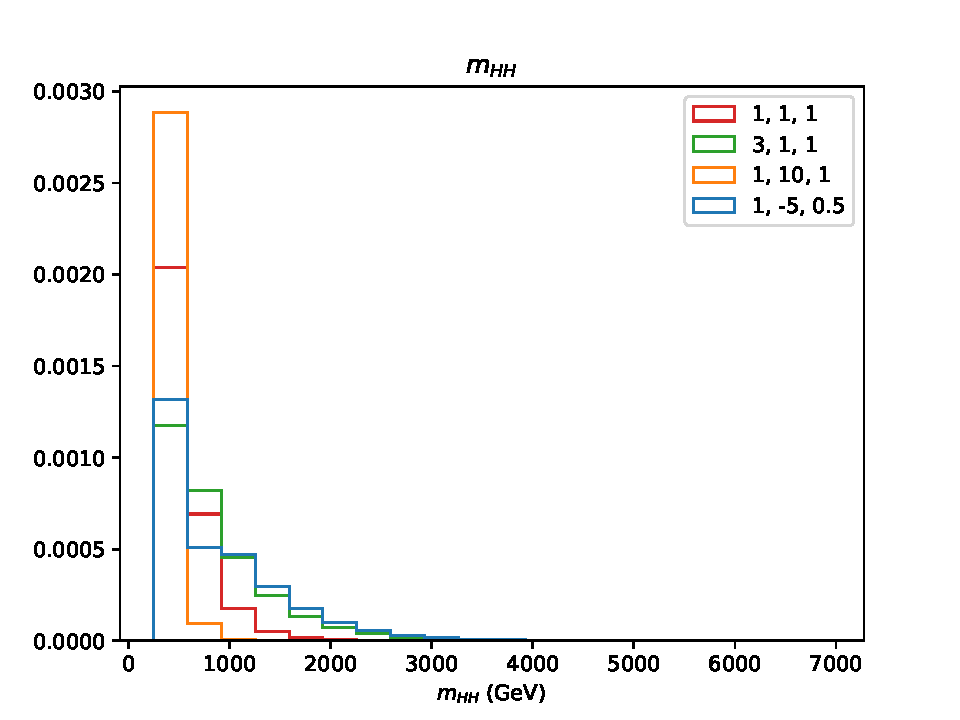
\includegraphics[width=\linewidth,height=\textheight,keepaspectratio]{signal/truth_lhe_HH_m}
            \captionsetup{justification=centering} \caption{Di-Higgs Invariant Mass}
        \end{subfigure}
        \begin{subfigure}{0.48\textwidth}
            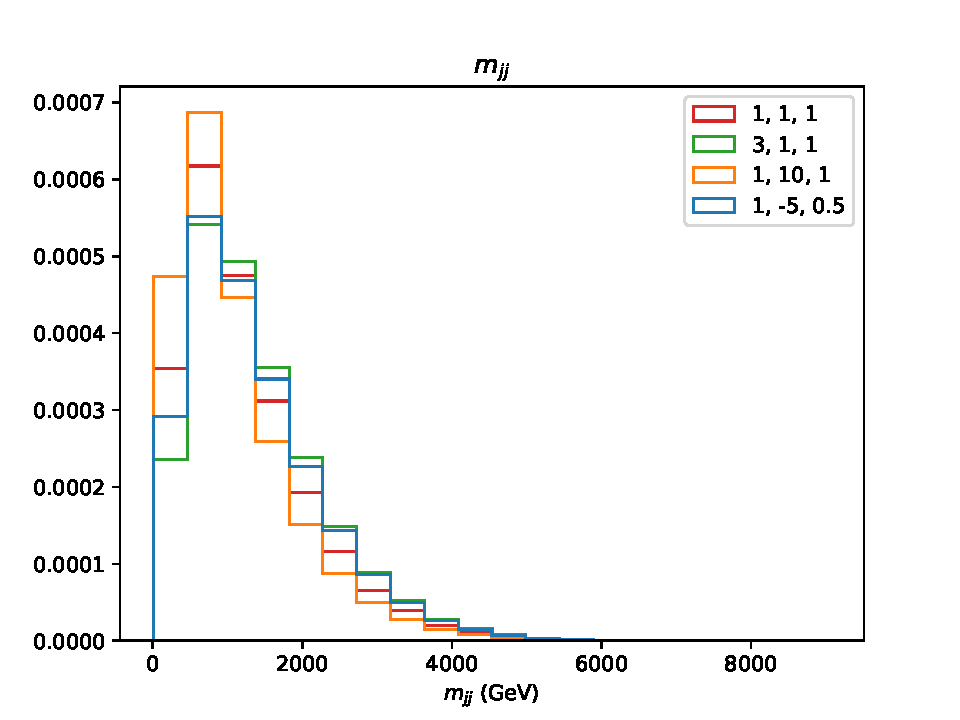
\includegraphics[width=\linewidth,height=\textheight,keepaspectratio]{signal/truth_lhe_jj_M}
            \captionsetup{justification=centering} \caption{VBF Initial Scatter Jets Invariant Mass}
        \end{subfigure}
        \caption{
            MC event distributions from \textit{truth-level} events.
            That is, events generated from MadGraph+Pythia8
                but which have not gone through Geant4 detector simulation or reconstruction.
            These plots show the invariant mass between the Higgs pair and VBF initial scatter jets respectively,
                for a number of different $\kappa$ scale factors.
        }
        \label{fig:lhe_truth1}
    \end{figure}

    \begin{figure}[tbh]
        \centering
        \begin{subfigure}{0.48\textwidth}
            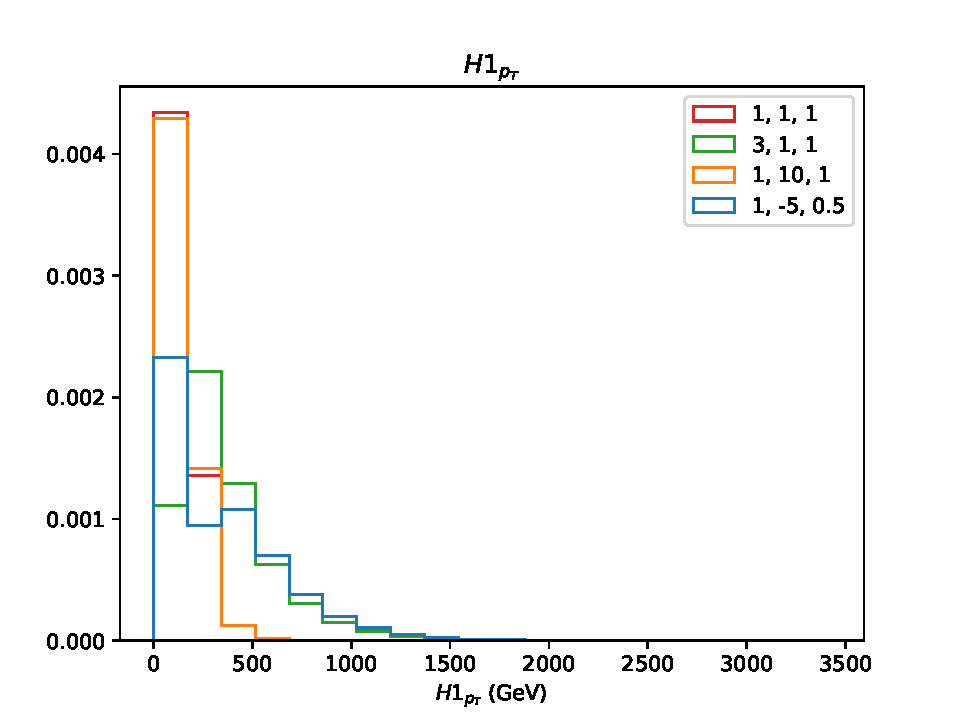
\includegraphics[width=\linewidth,height=\textheight,keepaspectratio]{signal/truth_lhe_H1_pt}
            \captionsetup{justification=centering} \caption{
                $p_T$ of the leading-$p_T$ Higgs boson
            }
        \end{subfigure}
        \begin{subfigure}{0.48\textwidth}
            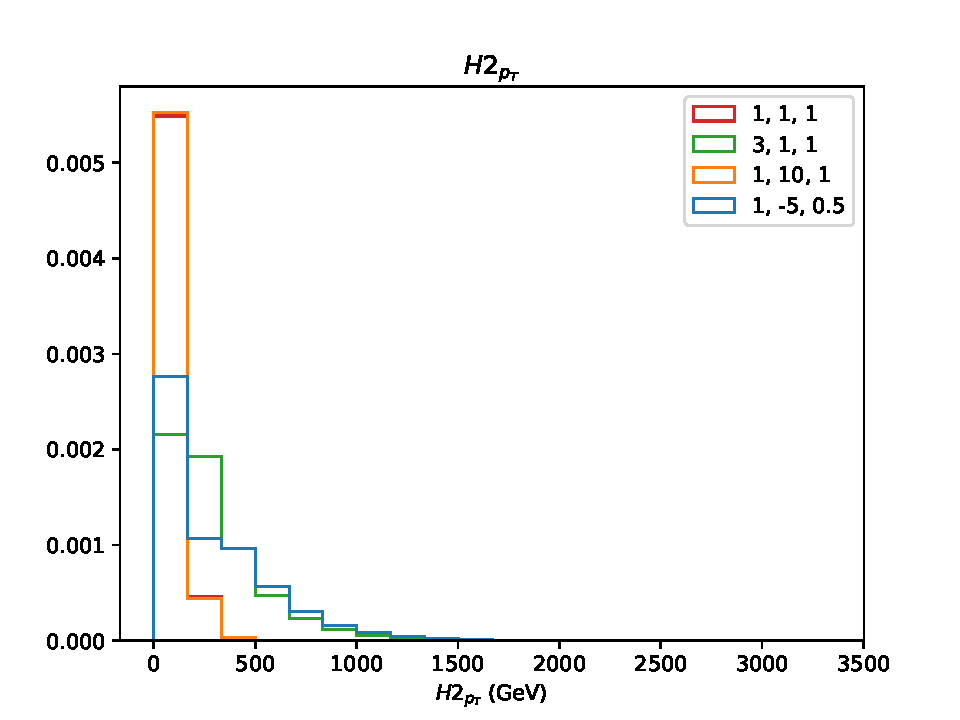
\includegraphics[width=\linewidth,height=\textheight,keepaspectratio]{signal/truth_lhe_H2_pt}
            \captionsetup{justification=centering} \caption{
                $p_T$ of the sub-leading-$p_T$ Higgs boson
            }
        \end{subfigure} \\

        \begin{subfigure}{0.48\textwidth}
            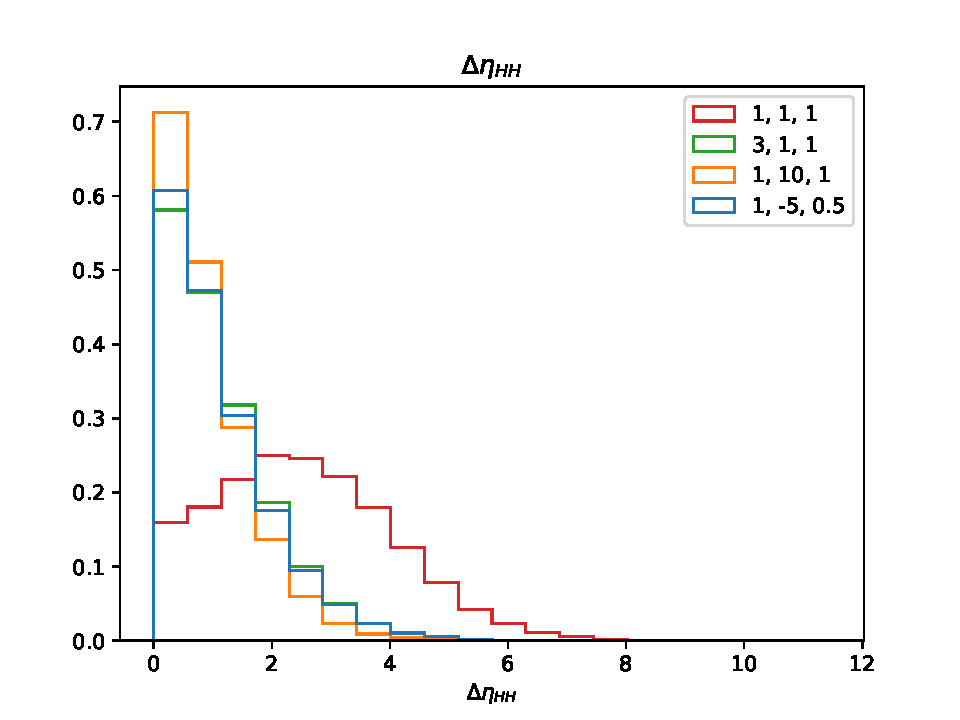
\includegraphics[width=\linewidth,height=\textheight,keepaspectratio]{signal/truth_lhe_HH_dEta}
            \captionsetup{justification=centering} \caption{
                \deta between the two produced Higgs bosons
            }
        \end{subfigure} \\
        \caption{
                Truth-level display of additional kinematic properties the \vbfhhproc.
        }
        \label{fig:lhe_truth2}
    \end{figure}

    Instead, a more robust hypothesis can be constructed by choosing an observable quantity distinct to the process in question.
    Here, the observable used is the invariant mass of the di-Higgs system (\mhh).
    The advantage of using \mhh is that the probability density function (PDF) for the \mhh of an event
        is predicted to vary significantly based on the values of the $\kappa$ scaling factors.
    As such, the shape of the PDF for \mhh is unique to particular values of the scale factors, 
        and so can be used to test the validity of a hypothesis.
    If the \mhh distribution reconstructed from the data collected at ATLAS has no resemblance to
        the \mhh distribution predicted for a particular combination of the scale factors,
        then that set of scale factors can be ruled out as incompatible with data
        at some level of statistical confidence
        (to be further discussed in Chapter \ref{chapter:results}).

    Of course, making a prediction for the shape of the \mhh distribution as it would appear in ATLAS is easier said than done.
    Calculating the event yield alone is not too difficult to perform by hand,
        as this requires only the cross-section of the process.
    Calculating the event yield as a function of an observable kinematic variable is much more difficult,
        requiring the differential cross-section $\dxsec{q_i}$.
    Section \ref{sec:mcsim} describes the Monte-Carlo simulation procedure used for this purpose,
        providing a model of how the kinematic distributions of the \vbfhhproc process would appear after passing through
        the ATLAS detector and the event selection process.
    The challenge addressed in this chapter then is with regard to the poorly defined range of the kappa coupling coefficients,
        and the variety of signal hypotheses this range entails.
    Modelling such a range accurately and efficiently necessitates revisiting the fundamental behaviour
        of the \hhproc process, and constitutes the bulk of my contribution to the 4b analysis.


\section{Signal Combination} \label{sec:signal_combination}

    As discussed in Section \ref{sec:feyn_rules},
        the cross-section and kinematic distributions of the di-Higgs production processes
        depend fundamentally on a number of scaling factors between the Higgs and other particles.
    Of particular interest in this analysis are \kl for the Higgs's self-coupling scale factor and \kvv for the \HHVV coupling scale factor.
    The values of \kl and \kvv have loose experimental constraints \cite{EXOT-2016-31} \cite{HDBS-2018-18-witherratum} \cite{ATLAS-CONF-2019-049},
        requiring analysis across a wide range of these scale factor values.
    Unfortunately, the MC generation process discussed in Section \ref{sec:mcsim} is computationally expensive and time consuming.
    As such, only a handful of MC simulation samples for a select few scale factor values are actually produced.
    A sample combination technique 
        (expanded upon from an analogous approach used in Ref. \cite{combination_origin})
        is employed to model the signal hypothesis across the scale factor parameter space.

    The process of combining a few samples in such a way as to model the entire parameter space of scaling factors
        is based on exploiting the underlying mathematics of the differential cross-section formula.
    By expanding the squared term of the sum of all Feynman diagram contributions,
        the cross-section can be expressed as a function of its scale factor values \cite{ATLAS-CONF-2019-049},
        as shown in Eqn. \ref{eq:tree_level_invamp}.
    Rewriting the expression again in terms of the differential cross-section as a function of the observable \mhh:
    \begin{equation} \begin{split} \label{eq:tree_level_invamp_simple}
        \xsec &\equiv \dXsecM \propto |\invAmp|^2 = |  \kv^2 M_t + \kv \kl M_s + \kvv M_x |^2 \\
        \xsec &= \kv^2 \kl^2 a_1 + \kv^4 a_2 + \kvv^2 a_3 + \kv^3 \kl a_4 + \kv \kl \kvv a_5 + \kv^2 \kvv a_6
        \,.
    \end{split} \end{equation}

    \newcommand{\crossterm}[1]{
        \xsec_{#1} &= \fkv{#1}^2 \fkl{#1}^2 a_1
            + \fkv{#1}^4 a_2
            + \fkvv{#1}^2 a_3
            + \fkv{#1}^3 \fkl{#1} a_4
            + \fkv{#1} \fkl{#1} \fkvv{#1} a_5
            + \fkv{#1}^2 \fkvv{#1} a_6
    }
    %\newcommand{\combterm}[1]{ g_{#1} \frac{d\sigma_{#1}}{d \mhh} }
    \newcommand{\combterm}[1]{ g_{#1} \xsec_{#1} }

    The $a_i$ matrix element expansion values have a dependence on \mhh, which is not trivially derivable as an analytic function.
    Instead, for a given scale factor,
        its cross-section for a given \mhh can be mathematically determined by solving a set of linear equations for the $a_i$ terms.
    This is done using six different cross-section values (for the same \mhh) for six different scaling values.

    %\begin{equation} \label{eq:allsixxsecs} \begin{aligned}
    %\begin{equation} \crossterm{1} \nonumber \end{equation}
    %\begin{equation} \crossterm{2} \nonumber \end{equation}
    %\begin{equation} \crossterm{3} \nonumber \end{equation}
    %\begin{equation} \crossterm{4} \nonumber \end{equation}
    %\begin{equation} \crossterm{5} \nonumber \end{equation}
    %\begin{equation} \label{eq.allsixxsecs} \crossterm{6} \,. \end{equation}
    %\end{aligned} \end{equation}

    \begin{eqnarray} \label{eq:allsixxsecs}
        \crossterm{1} \nonumber \\
        \crossterm{2} \nonumber \\
        \crossterm{3} \nonumber \\
        \crossterm{4} \nonumber \\
        \crossterm{5} \nonumber \\
        \crossterm{6} \nonumber \,. \\
    \end{eqnarray}

    This set of equations can be reformatted as a matrix equation
        by rewriting the differential cross-sections and $a_i$ terms as vectors,
    \begin{equation}
        \vec{\xsec} = \minimatrix{ \xsec_{1} \\ \xsec_{2} \\ \xsec_{3} \\ \xsec_{4} \\ \xsec_{5} \\ \xsec_{6} }
        \qquad,\qquad
        \vec{a} = \minimatrix{ a_1 \\ a_2 \\ a_3 \\ a_4 \\ a_5 \\ a_6 }
        \,.
    \end{equation}
    By reformatting the various $\kappa$ terms as a vector function $\vec{f}$,
        the collection of varied scale factors can be written as a matrix $F$
    \begin{equation}
        \vec{f} = \begin{pmatrix} \kv^2 \kl^2 \\ \kv^4 \\ \kvv^2 \\ \kv^3 \kl \\ \kv \kl \kvv \\ \kv^2 \kvv \end{pmatrix}
        \quad,\quad
        F = \begin{pmatrix}
            \vec{f}(\fkvv{1}, \fkl{1}, \fkv{1}) \\
            \vec{f}(\fkvv{2}, \fkl{2}, \fkv{2}) \\
            \vec{f}(\fkvv{3}, \fkl{3}, \fkv{3}) \\
            \vec{f}(\fkvv{4}, \fkl{4}, \fkv{4}) \\
            \vec{f}(\fkvv{5}, \fkl{5}, \fkv{5}) \\
            \vec{f}(\fkvv{6}, \fkl{6}, \fkv{6}) \\
        \end{pmatrix}
        \,.
    \end{equation}

    Equation \ref{eq:allsixxsecs} can then be written in the much simpler form
    \begin{equation}
        \vec{\xsec} = F \bullet \vec{a}
        \,.
    \end{equation}
    The $a_i$ terms can then be trivially solved for through an inversion of $F$
    \begin{equation} \label{eq:amp_solution}
        \vec{a} = F^{-1} \bullet \vec{\xsec}
        \,.
    \end{equation}
    Substituting \ref{eq:amp_solution} back into \ref{eq:tree_level_invamp_simple} produces
        a final expression for deriving a combined differential cross-section $\xsec'$ of the form
    \begin{equation} \label{eq:combination_general} \begin{split}
        \xsec'(\kvv,\kl,\kv) &= \vec{f}(\kvv,\kl,\kv) \bullet \vec{a}
            = \vec{f}(\kvv,\kl,\kv) \bullet F^{-1} \bullet \vec{\xsec} \\
        \xsec'(\kvv,\kl,\kv) &= \vec{g}(\kvv,\kl,\kv) \bullet \vec{\xsec}
            \quad,\quad \vec{g} \equiv \vec{f}(\kvv,\kl,\kv) \bullet F^{-1} \\
        \xsec'(\kvv,\kl,\kv) &= 
            \combterm{1} +
            \combterm{2} +
            \combterm{3} +
            \combterm{4} +
            \combterm{5} +
            \combterm{6}
        \,.
    \end{split} \end{equation}

    In practice, the differential cross-section values $\xsec_i$ of these six \textit{basis} samples
        are represented by their yields from MC simulation,
        binned by their \mhh values,
        which are added together after being multiplied by their respective combination coefficient $g_i$.
    Due to the complexities of the kinematics of the VBF process,
        the samples used in the combination must have already been run through the full reconstruction and selection process detailed in Section \ref{sec:mcsim}.
    The signal distribution modeling is thus performed by directly combining the reconstructed \mhh distributions of post-selection signal samples.

    \begin{table}[] \centering
    \caption{6-Term VBF Combination Sample Variations.}
    \label{tab:vbf_hh_6term_varlist}
    \begin{tabular}{ |l|l|l| }
        \hline
        \textbf {$\kappa_{2V}$} & \textbf {$\kappa_\lambda$} & \textbf {$\kappa_V$} \\
        \hline
            1   &   1 & 1   \\
            1.5 &   1 & 1   \\
            1   &   2 & 1   \\
            1   &  10 & 1   \\
            1   &   1 & 0.5 \\
            0   &  -5 & 0.5 \\
        \hline
    \end{tabular} \end{table}

    In theory, with infinite events, the only requirement for these samples is that they are linearly independent of each other.
    In practice, the final samples are statistically limited, and different combinations of variations yield different statistical power.
    The 6-sample combination used in this analysis (Table \ref{tab:vbf_hh_6term_varlist} and Eqn. \ref{eqn:vbf_hh_6term_chosen}) has been chosen specifically for its ability to avoid mis-modeling errors.

    {\footnotesize \begin{equation}
    \label{eqn:vbf_hh_6term_chosen}
    \begin{split}
        \xsec'(\kvv, \kl, \kv) =
        \left(\frac{68 \kappa_{2V}^{2}}{135} - 4 \kappa_{2V} \kappa_{V}^{2} + \frac{20 \kappa_{2V} \kappa_{V} \kappa_{\lambda}}{27} + \frac{772 \kappa_{V}^{4}}{135} - \frac{56 \kappa_{V}^{3} \kappa_{\lambda}}{27} + \frac{\kappa_{V}^{2} \kappa_{\lambda}^{2}}{9}\right)
            \times & \xsec{\left(1,1,1 \right)} \\
        + \left(- \frac{4 \kappa_{2V}^{2}}{5} + 4 \kappa_{2V} \kappa_{V}^{2} - \frac{16 \kappa_{V}^{4}}{5}\right)
            \times & \xsec{\left(\frac{3}{2},1,1 \right)} \\
        + \left(\frac{11 \kappa_{2V}^{2}}{60} + \frac{\kappa_{2V} \kappa_{V}^{2}}{3} - \frac{19 \kappa_{2V} \kappa_{V} \kappa_{\lambda}}{24} - \frac{53 \kappa_{V}^{4}}{30} + \frac{13 \kappa_{V}^{3} \kappa_{\lambda}}{6} - \frac{\kappa_{V}^{2} \kappa_{\lambda}^{2}}{8}\right)
            \times & \xsec{\left(1,2,1 \right)} \\
        + \left(- \frac{11 \kappa_{2V}^{2}}{540} + \frac{11 \kappa_{2V} \kappa_{V} \kappa_{\lambda}}{216} + \frac{13 \kappa_{V}^{4}}{270} - \frac{5 \kappa_{V}^{3} \kappa_{\lambda}}{54} + \frac{\kappa_{V}^{2} \kappa_{\lambda}^{2}}{72}\right)
            \times & \xsec{\left(1,10,1 \right)}  \\
        + \left(\frac{88 \kappa_{2V}^{2}}{45} - \frac{16 \kappa_{2V} \kappa_{V}^{2}}{3} + \frac{4 \kappa_{2V} \kappa_{V} \kappa_{\lambda}}{9} + \frac{152 \kappa_{V}^{4}}{45} - \frac{4 \kappa_{V}^{3} \kappa_{\lambda}}{9}\right)
            \times & \xsec{\left(1,1,\frac{1}{2} \right)} \\
        + \left(\frac{8 \kappa_{2V}^{2}}{45} - \frac{4 \kappa_{2V} \kappa_{V} \kappa_{\lambda}}{9} - \frac{8 \kappa_{V}^{4}}{45} + \frac{4 \kappa_{V}^{3} \kappa_{\lambda}}{9}\right)
            \times & \xsec{\left(1,-5,\frac{1}{2} \right)}
        \,.
    \end{split} \end{equation}}

    The method used to determine the overall performance of a basis is to check the number of negative bins generated
        in the \mhh distribution across all points in the two-dimensional \kvv,\kl space, as seen in Fig. \ref{fig:vbf_hh_6term_nWeight_grid}.
    As negative bin weights are unphysical, they indicate poor signal modeling.
    Thus, identifying a basis which minimizes the presence of negative weights
        ensures stable modeling of the signal hypothesis at all points in the coupling space
        (Figs. \ref{fig:vbf_hh_6term_validation} and \ref{fig:vbf_hh_6term_preview}).

    \begin{figure}[tbh]
        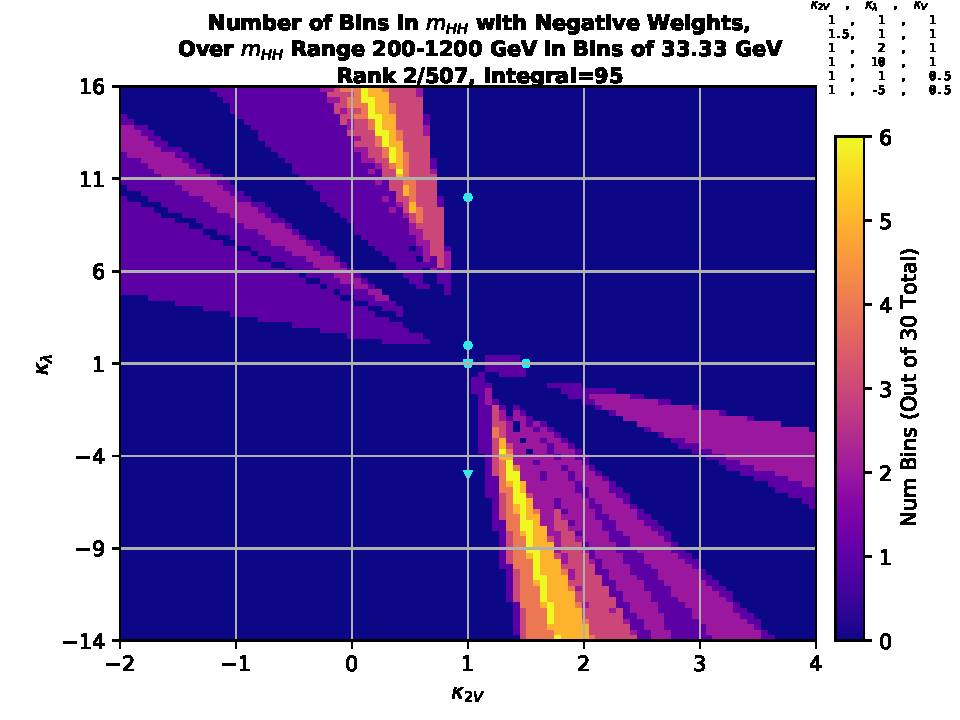
\includegraphics[width=\linewidth,height=\textheight,keepaspectratio]{signal/negative_weights_base}
        \caption{
            Frequency of negative bin weights in \mhh distribution across \kvv,\kl range.
            Brighter regions indicate more negative-weighted bins, and suggest less stable signal modeling.
            This particular combination of samples was chosen for how much of the space is ``dark,''
                with darker regions indicating generally stable signal modeling.
            The table of coupling values in the upper right corner indicates the 6 MC samples
                (highlighted on the plot with cyan dots) used in the combination.
        }
        \label{fig:vbf_hh_6term_nWeight_grid}
    \end{figure}

    Ultimately however, the final arbiter of a well constructed basis is that it produces observable distributions comparable to what would be produced through direct MC generation.
    A number of validation tests are thus performed, comparing the distributions from the combination to an already existing MC sample.
    Displayed in Fig. \ref{fig:vbf_hh_6term_validation}, the combination shows strong agreement with the MC sample.

    \begin{figure}[tbh]
        \begin{subfigure}{0.48\textwidth}
            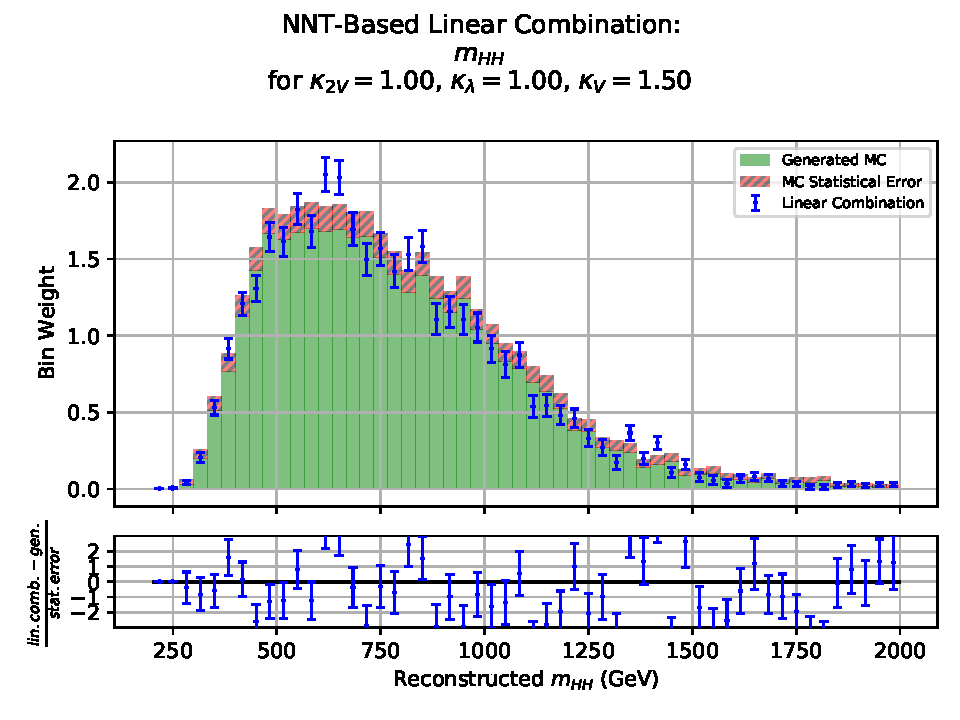
\includegraphics[width=\linewidth,height=\textheight,keepaspectratio]{signal/reco_mHH_cvv1p00cl1p00cv1p50}
            \captionsetup{justification=centering} \caption{Validation \kv = 1.5}
        \end{subfigure}
        \begin{subfigure}{0.48\textwidth}
            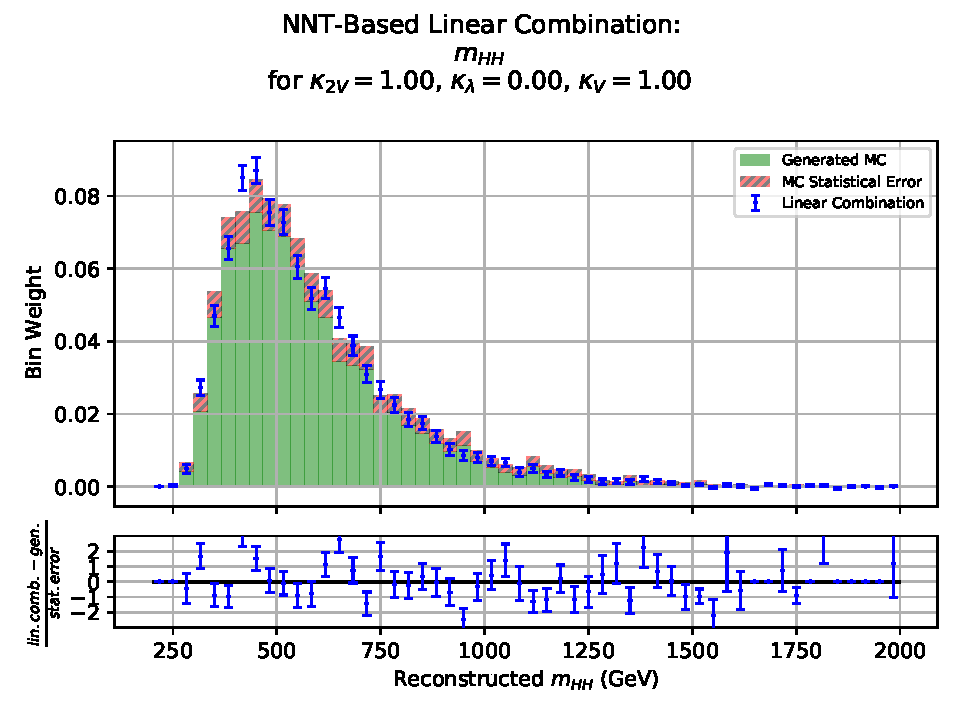
\includegraphics[width=\linewidth,height=\textheight,keepaspectratio]{signal/reco_mHH_cvv1p00cl0p00cv1p00}
            \captionsetup{justification=centering} \caption{Validation \kl = 0}
        \end{subfigure}
        \caption{
            Validation of 6-term combination against MC generated at \kv = 1.5 and \kl = 0.
            The combination shows good agreement to the generated MC distributions.
        }
        \label{fig:vbf_hh_6term_validation}
    \end{figure}

    \begin{figure}[tbh]
    	\centering
        \begin{subfigure}{0.32\textwidth}
            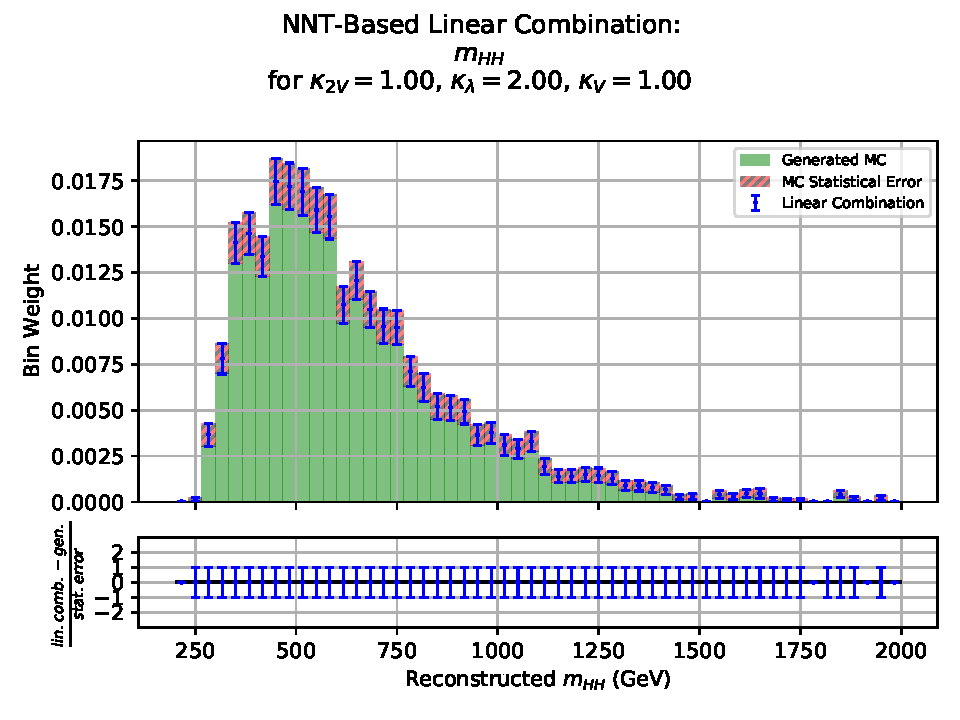
\includegraphics[width=\linewidth,height=\textheight,keepaspectratio]{signal/reco_mHH_cvv1p00cl2p00cv1p00}
            \captionsetup{justification=centering} \caption{Validation against MC with $\kl=2$}
        \end{subfigure}
        \begin{subfigure}{0.32\textwidth}
            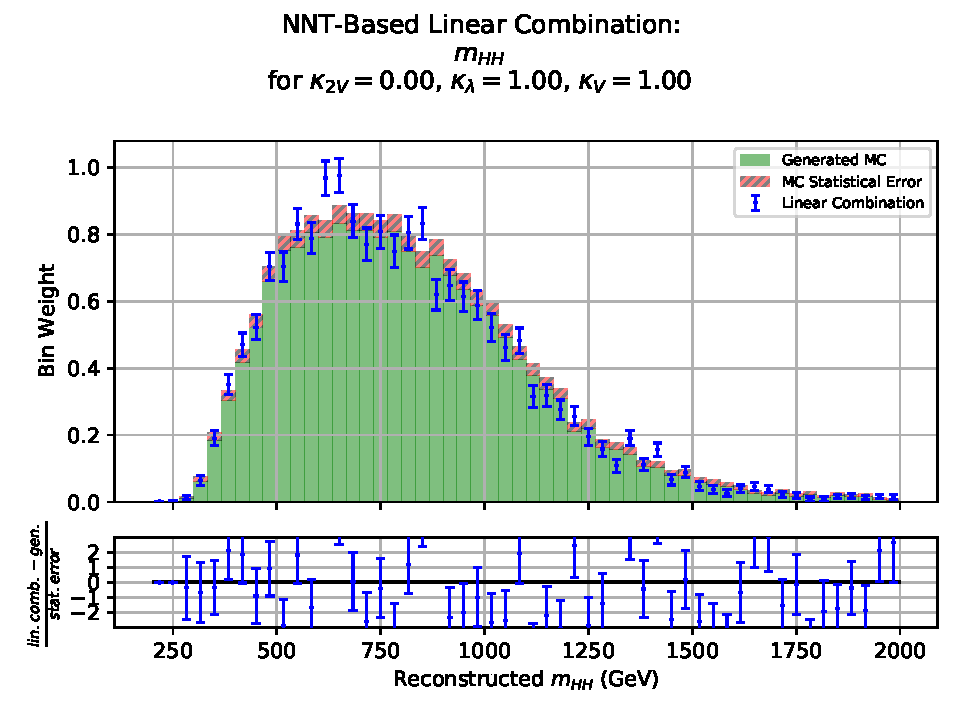
\includegraphics[width=\linewidth,height=\textheight,keepaspectratio]{signal/reco_mHH_cvv0p00cl1p00cv1p00}
            \captionsetup{justification=centering} \caption{Validation against MC with $\kvv=0$}
        \end{subfigure}
        \begin{subfigure}{0.32\textwidth}
            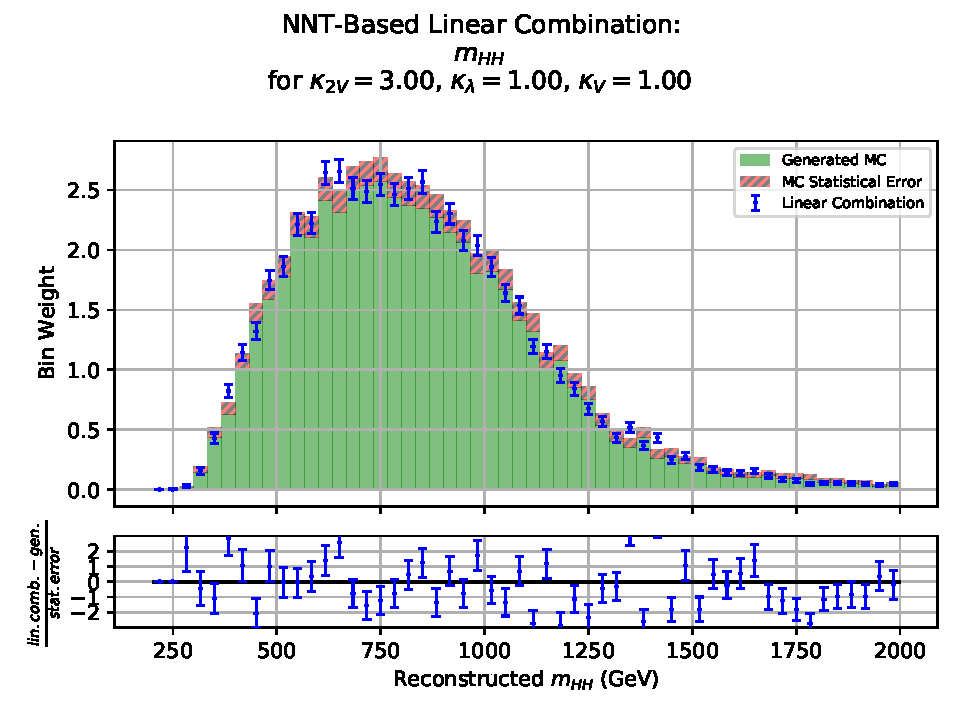
\includegraphics[width=\linewidth,height=\textheight,keepaspectratio]{signal/reco_mHH_cvv3p00cl1p00cv1p00}
            \captionsetup{justification=centering} \caption{Validation against MC with $\kvv=3$}
        \end{subfigure}
        \caption{
            The six-term linear combination of samples is combined for various coupling scaling factor values.
            The combined distribution shape (in blue) is compared against a Monte-Carlo sample (in green)
                which was generated for the same coupling scaling factor values.
            The combination approach shows good agreement with the generated sample, indicating accurate modeling of the signal shape.
        }
        \label{fig:vbf_hh_validation}
    \end{figure}

    As an additional test, I also checked the distribution shape predicted by the combination at points far from the SM.
    These points have no MC samples to compare to, but the points can still be checked to ensure they at least appear well-behaved.

    \begin{figure}[tbh]
        \centering
        \begin{subfigure}{0.32\textwidth}
            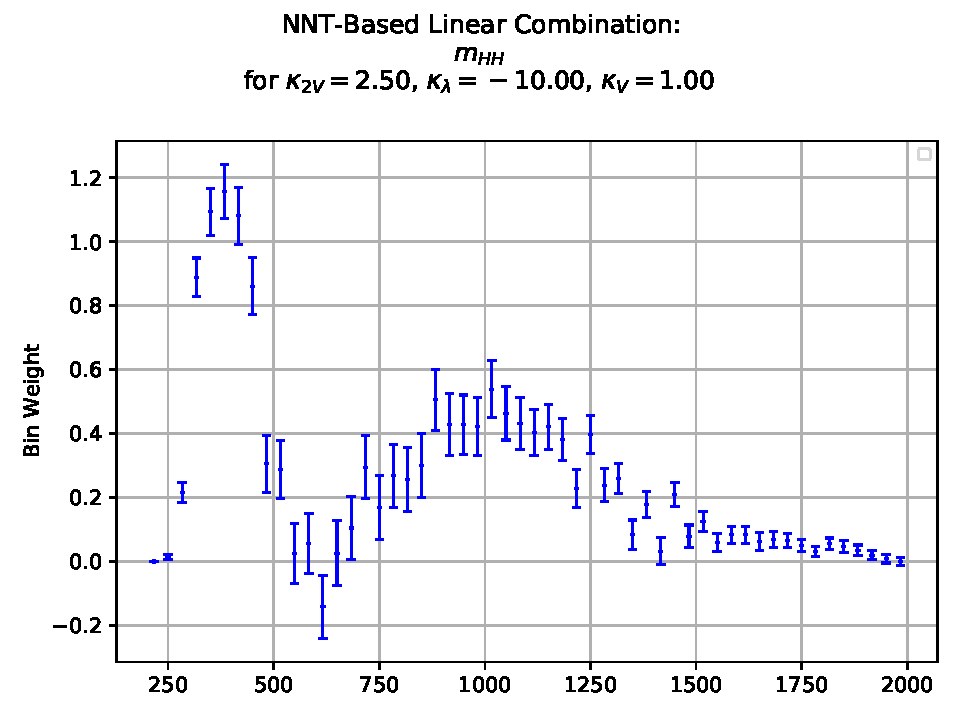
\includegraphics[width=\linewidth,height=\textheight,keepaspectratio]{signal/preview_reco_mHH_new_cvv2p50cl-10p00cv1p00}
            \captionsetup{justification=centering} \caption{Combined \mhh distribution at \kvv = 2.5, \kl = -10}
        \end{subfigure}
        \begin{subfigure}{0.32\textwidth}
            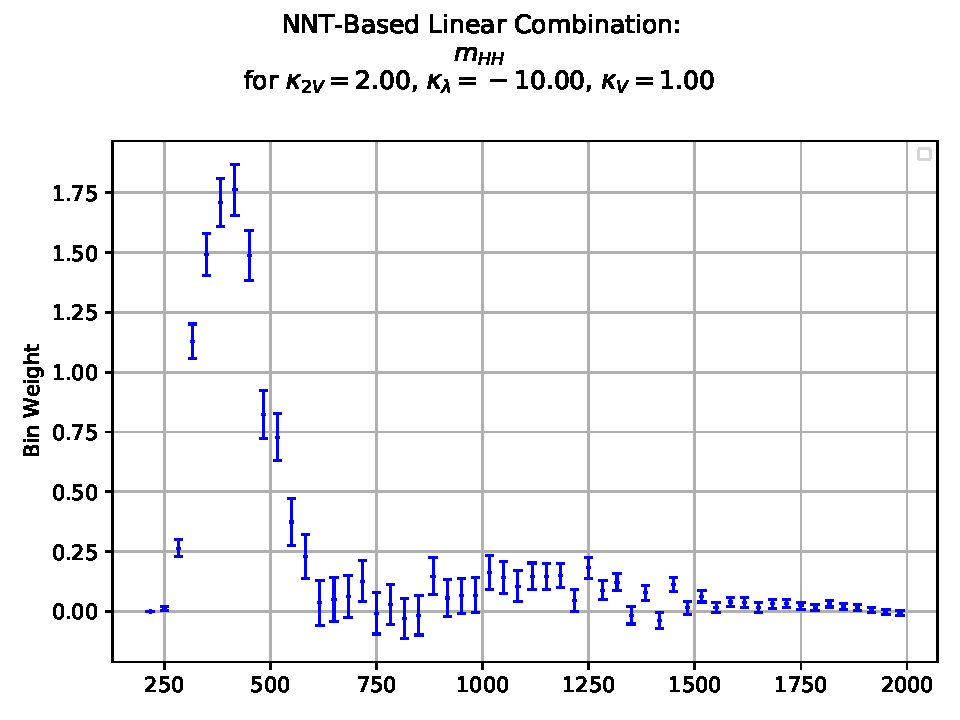
\includegraphics[width=\linewidth,height=\textheight,keepaspectratio]{signal/preview_reco_mHH_new_cvv2p00cl-10p00cv1p00}
            \captionsetup{justification=centering} \caption{Combined \mhh distribution at \kvv = 2.0, \kl = -10}
        \end{subfigure}
        \begin{subfigure}{0.32\textwidth}
            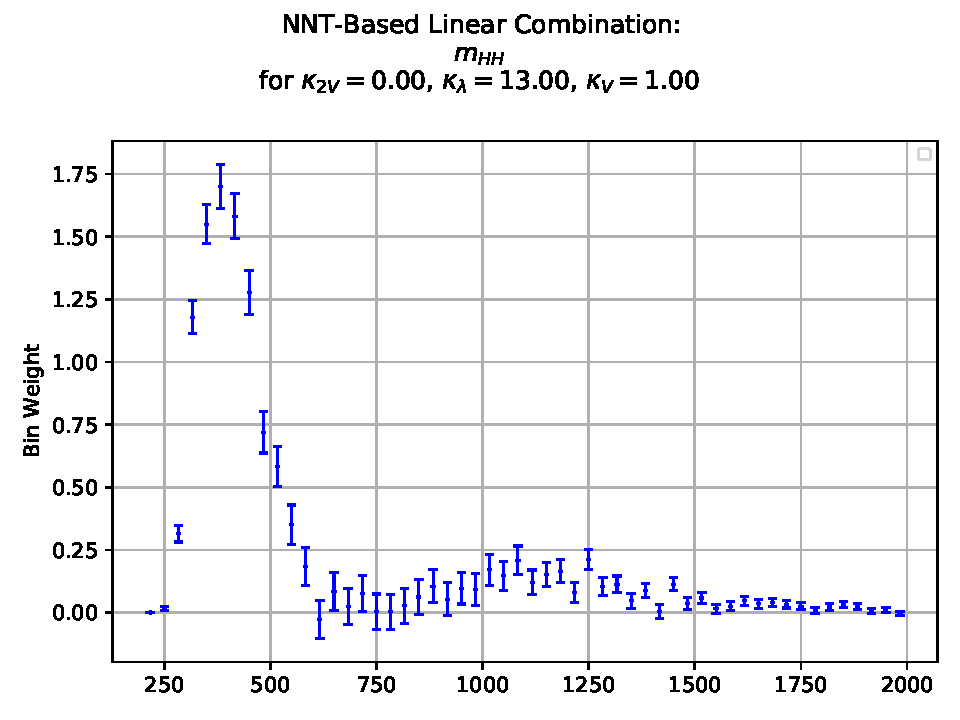
\includegraphics[width=\linewidth,height=\textheight,keepaspectratio]{signal/preview_reco_mHH_new_cvv0p00cl13p00cv1p00}
            \captionsetup{justification=centering} \caption{Combined \mhh distribution at \kvv = 0, \kl = 13}
        \end{subfigure}
        \caption{
            \mhh distribution produced by the 6-term combination at points far from the SM.
            The combination produces smooth, well-behaved distributions at these points,
                suggesting the signal is well-modeled in these regions.
        }
        \label{fig:vbf_hh_6term_preview}
    \end{figure}

    \begin{figure}[tbh]
    	\centering
        \begin{subfigure}{0.44\textwidth}
            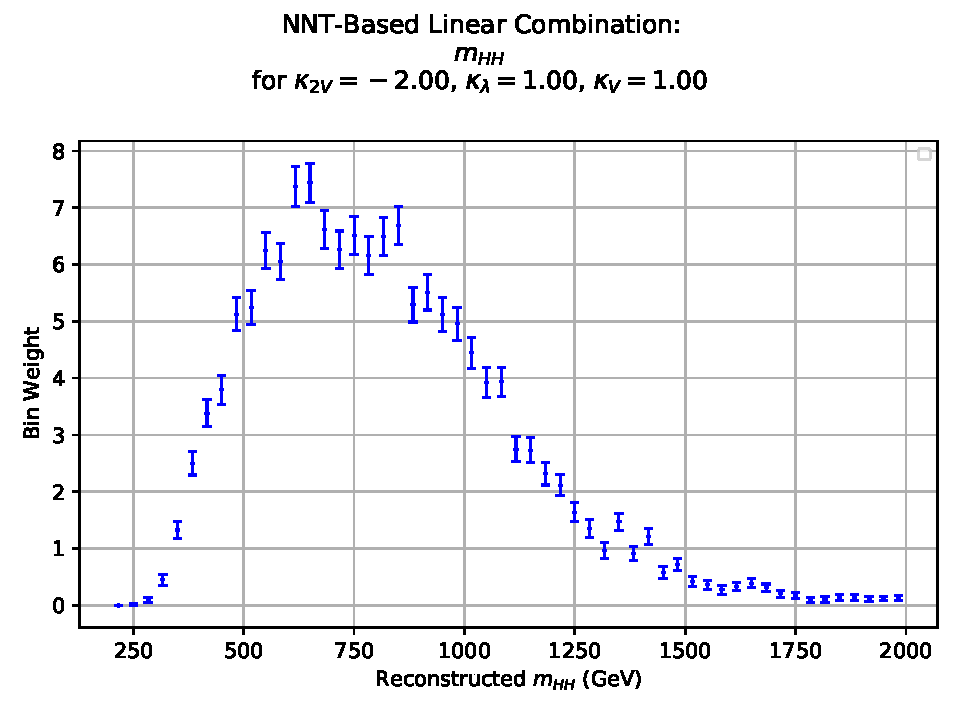
\includegraphics[width=\linewidth,height=\textheight,keepaspectratio]{signal/preview_reco_mHH_new_cvv-2p00cl1p00cv1p00}
            \captionsetup{justification=centering} \caption{Combination at  \kvv = -2}
        \end{subfigure}
        \begin{subfigure}{0.44\textwidth}
            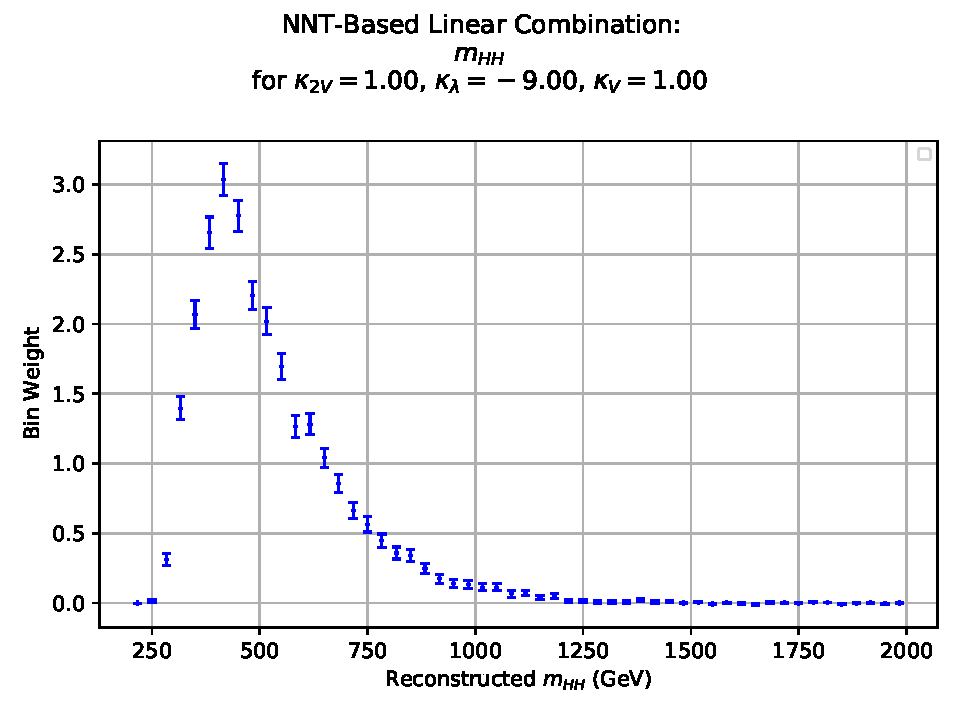
\includegraphics[width=\linewidth,height=\textheight,keepaspectratio]{signal/preview_reco_mHH_new_cvv1p00cl-9p00cv1p00}
            \captionsetup{justification=centering} \caption{Combination at  \kl = -9}
        \end{subfigure}
        \caption{
            The six-term linear combination of samples is combined for scale factor scaling factor values very far from the Standard Model.
            There are no MC simulated samples to compare these points too, but the combined distributions at these points are smooth and well-behaved,
                indicating reasonable modeling of the distribution even at distant scale factor scaling factors.
        }
        \label{fig:vbf_hh_preview}
    \end{figure}


\section{Solidarity} \label{sec:solidarity}
    
    As an additional note on the discussion of the signal sample combination technique,
        I would like to address the reason that some combination bases work better than others.
    Originally, the 2021 MC production for the 4b analysis consisted of 12 samples (all but the bottom row of Table \ref{tab:mcyields}).
    However, inspection of these samples using the negative weight technique discussed above revealed very poor modeling performance.
    From a combinatorics perspective, there were 12 samples available, and six are needed for the combination.
    There are 924 ways to choose 6 samples from 12, and of those 619 produce linearly solvable systems of equations.
    Of the 619, only 250 include the Standard Model MC sample.
    None of these 250 combination bases produced stable signal models across the $\kappa$-scale factor space.
    The performance of the two bases with the overall fewest number of negative bin weights is shown in Fig. \ref{fig:mcnWeight_old} and \ref{fig:mcpreviews_old}.

    \begin{figure}[tbh]
    	\centering
        \begin{subfigure}{0.44\textwidth}
            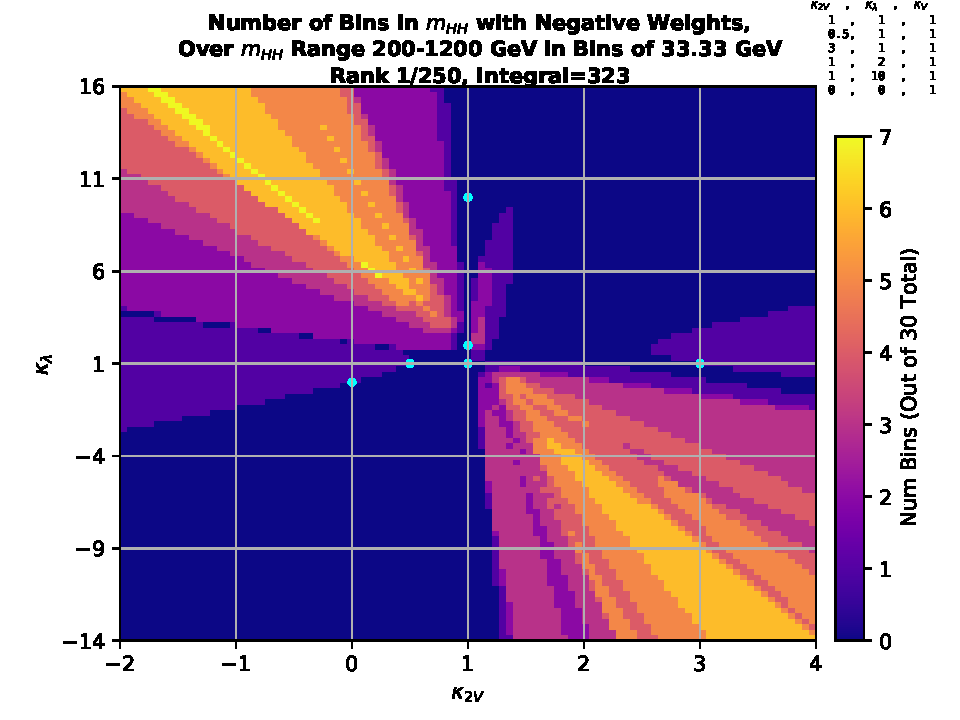
\includegraphics[width=\linewidth,height=\textheight,keepaspectratio]{signal/negative_weights_toprank0}
            \captionsetup{justification=centering} \caption{Original 12, Rank 1 negative weight heatmap}
        \end{subfigure}
        \begin{subfigure}{0.44\textwidth}
            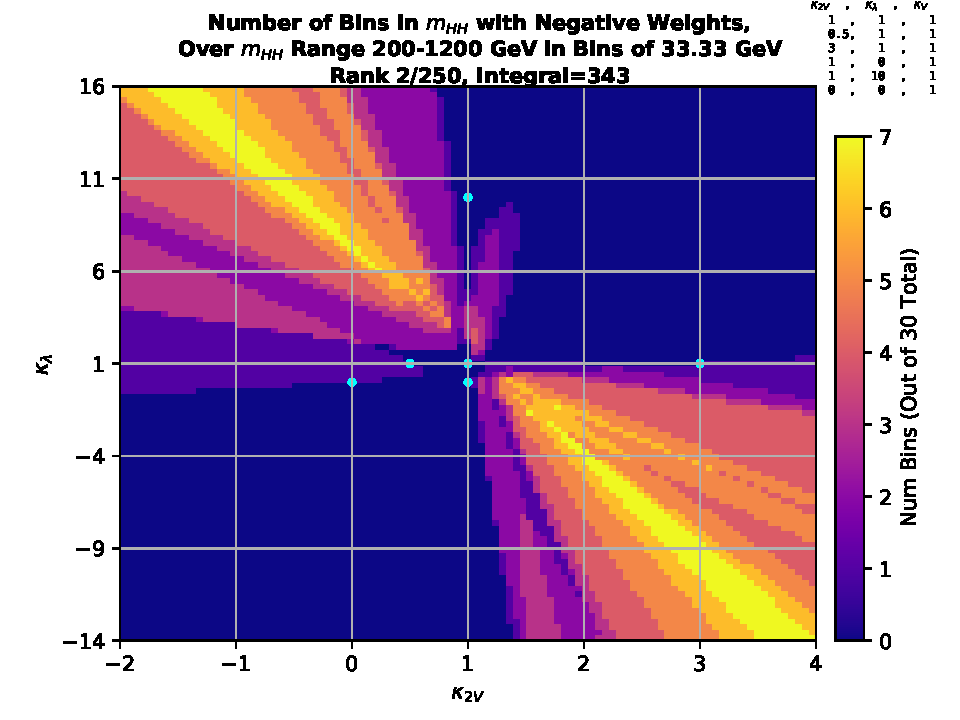
\includegraphics[width=\linewidth,height=\textheight,keepaspectratio]{signal/negative_weights_toprank1}
            \captionsetup{justification=centering} \caption{Original 12, Rank 2 negative weight heatmap}
        \end{subfigure}
        \caption{
            The two best performing bases of the original 12 MC samples.
            Both bases show a distressing abundance of negative weighted bins across a wide swath of the $\kappa$-scale factor space.
        }
        \label{fig:mcnWeight_old}
    \end{figure}


    \begin{figure}[tbh]
    	\centering
        \begin{subfigure}{0.44\textwidth}
            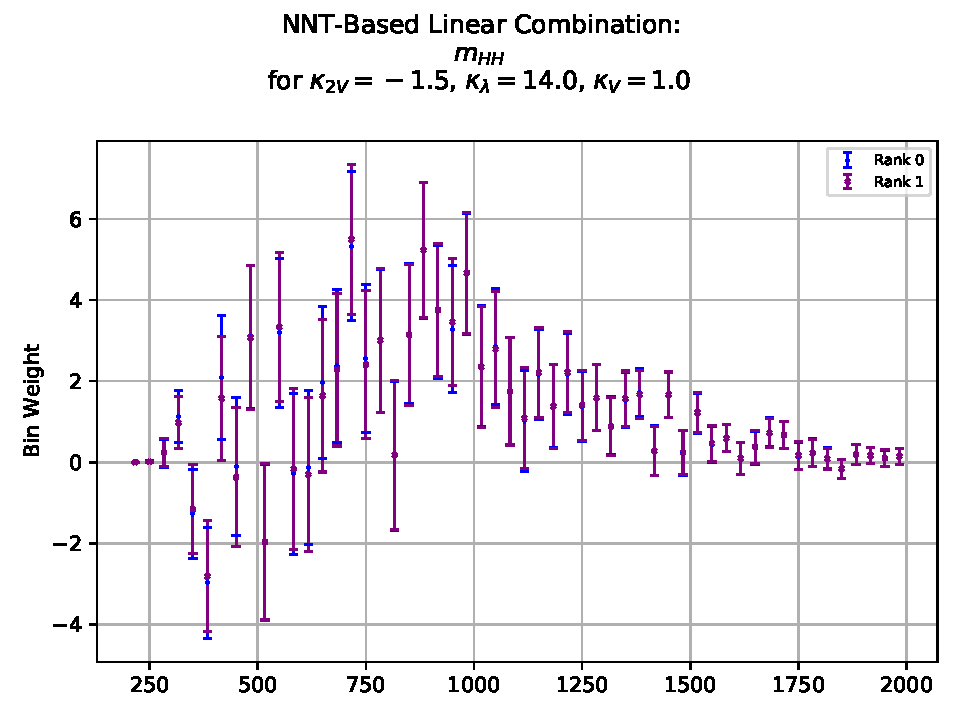
\includegraphics[width=\linewidth,height=\textheight,keepaspectratio]{signal/reco_mHH_compare_preview_auto_top_3D_0-1_cvv-1p5cl14p0cv1p0}
            \captionsetup{justification=centering} \caption{}
        \end{subfigure}
        \begin{subfigure}{0.44\textwidth}
            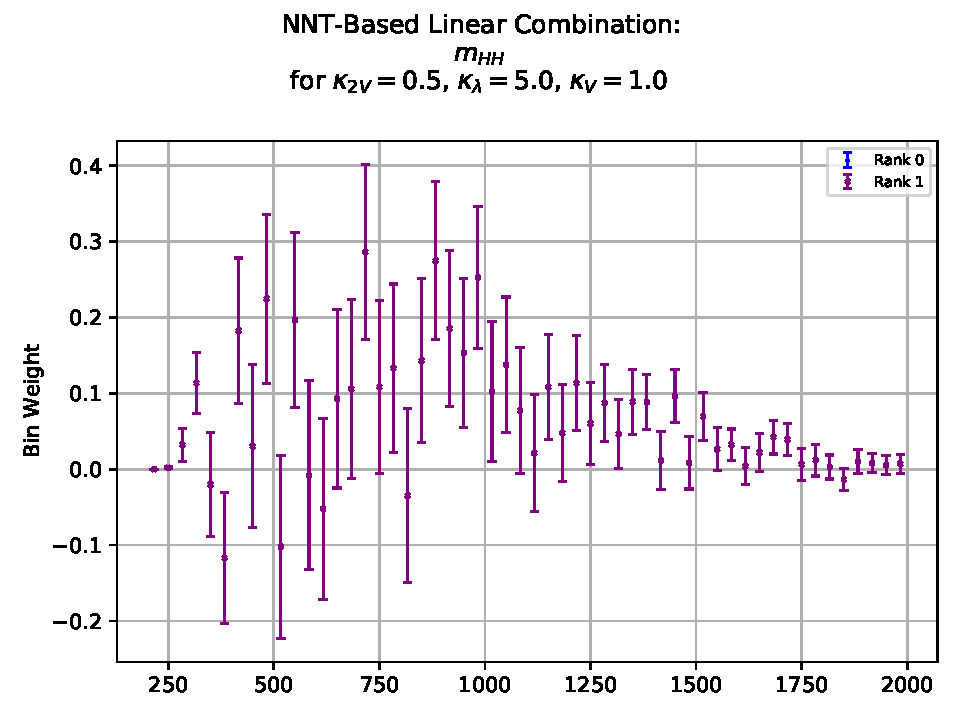
\includegraphics[width=\linewidth,height=\textheight,keepaspectratio]{signal/reco_mHH_compare_preview_auto_top_3D_0-1_cvv0p5cl5p0cv1p0}
            \captionsetup{justification=centering} \caption{}
        \end{subfigure}\\
        \begin{subfigure}{0.44\textwidth}
            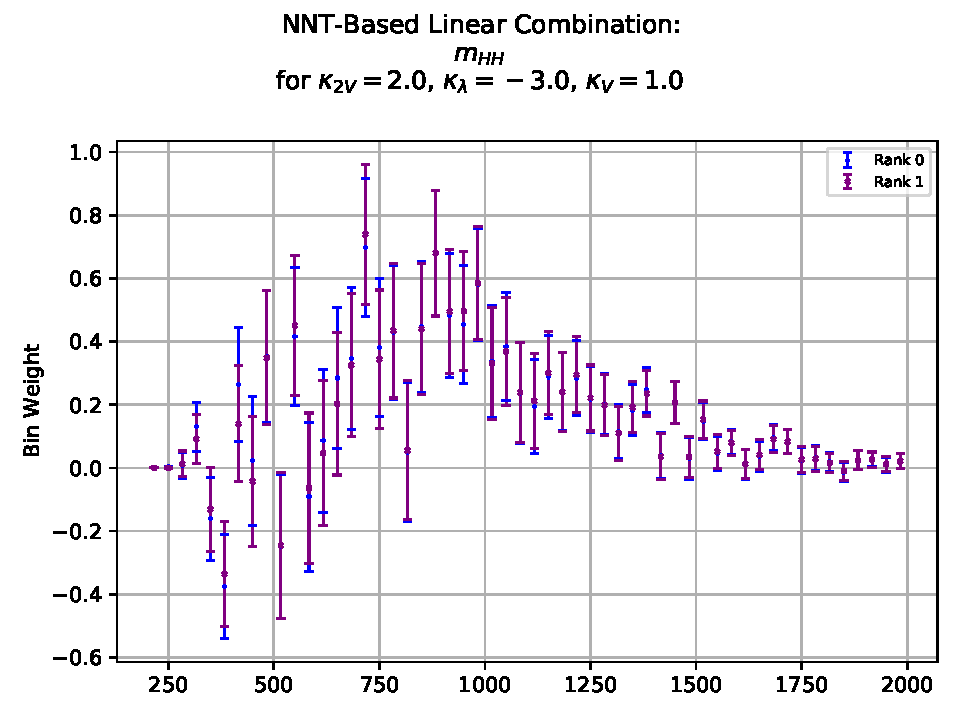
\includegraphics[width=\linewidth,height=\textheight,keepaspectratio]{signal/reco_mHH_compare_preview_auto_top_3D_0-1_cvv2p0cl-3p0cv1p0}
            \captionsetup{justification=centering} \caption{}
        \end{subfigure}
        \begin{subfigure}{0.44\textwidth}
            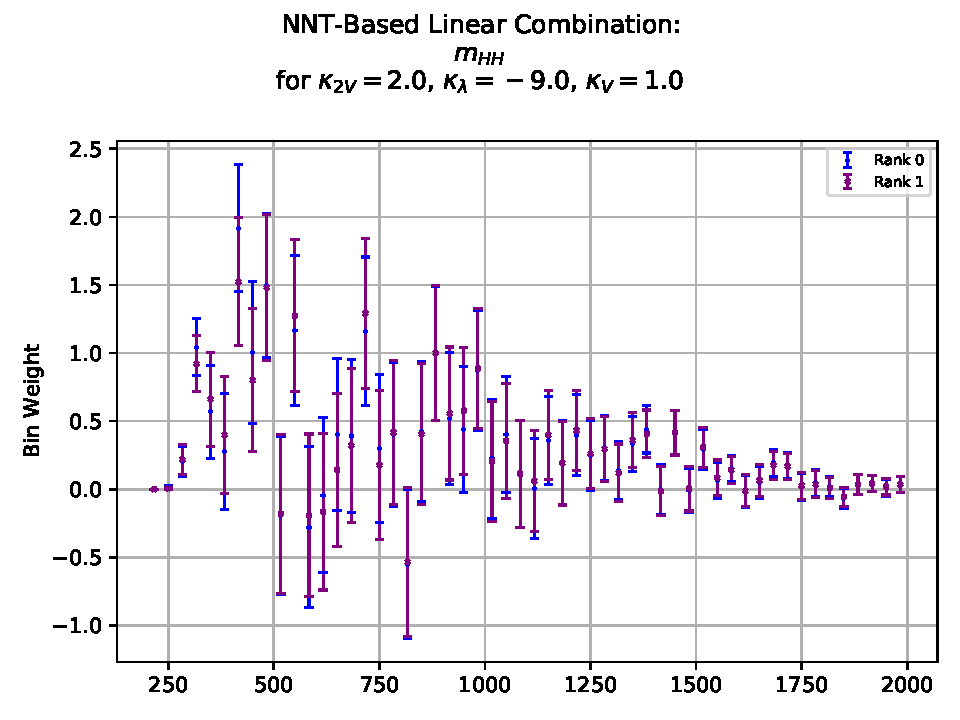
\includegraphics[width=\linewidth,height=\textheight,keepaspectratio]{signal/reco_mHH_compare_preview_auto_top_3D_0-1_cvv2p0cl-9p0cv1p0}
            \captionsetup{justification=centering} \caption{}
        \end{subfigure}
        \caption{
            The two best performing bases of the original 12 MC samples,
                modeling \mhh distributions for points far from the SM.
            Both bases produce very unstable distributions.
        }
        \label{fig:mcpreviews_old}
    \end{figure}


    The proposed solution was to generate one additional MC sample,
        which could be used in combination with five of the original samples to produce a stable basis.
    Of course, until the sample was produced, the negative weight optimization technique could not be used to assess the new sample's performance.
    As such, I developed a novel optimization metric which could predict the performance of a particular basis,
        without the need for any MC production.
    My hypothesis for the behavior of the sample combinations is that the regions of the scale factor space which perform poorly
        (e.g.\ the top left corners of Fig. \ref{fig:mcnWeight_old}),
        do so because one or two of the samples is disproportionately represented in the combination compared to the others.
    The formula for the combination of the samples (c.f.\ Eqn. \ref{eq:combination_general}) amounts to
        weighting each sample's differential cross-section $\xsec_i$ by a $\kappa$-factor-dependent coefficient $g_i(\kvv,\kl,\kv)$,
        and then adding these weighted cross-sections together to obtain the combined differential cross-section.
    Different samples can have cross-sections which are orders of magnitude apart from each other
        (e.g.\ the 1.18 fb cross-section of the SM point VS the 67 fb cross-section of the \kl=10 sample).
    As well, the $\kappa$-factor-based coefficients $g_i$ can vary dramatically across the $\kappa$ space.
    The product of the sample cross-section and the scale factor coefficient (the \textit{weighted cross-section})
        can therefore fluctuate a great deal across the scale factor space.
    For many regions of the $\kappa$ space, it can happen that one or two of the samples' weighted cross-sections vastly outweigh the others.
    In such cases, the combined cross-section is then based almost entirely on these one or two over-represented samples,
        making the combination much more susceptible to statistical deficiencies.
    I propose that this ``closeness'' of the weighted cross-sections can be used as an effective metric of performance
        and one which does not depend on the generation of MC.

    Here I define a metric to quantify this behavior.
    Due to the nature of the weighted cross-sections,
        the metric will be dependent both on the basis samples' cross-section ($\sigma_i$),
        and on the scale factor coefficient ($g_i(\kvv,\kl,\kv)$) of the specific point in the scale factor space to be modeled\footnote{
            Note that I have switched from a binned differential cross-section, to here working with the total cross-section.
            This is possible because the $g_i$ terms are independent of phase-space,
                and therefore do not affect the phase-space integration of the differential cross-section.
        }.
    As well, I want to explicitly note the occurrence of \textit{negative} coefficients in the combination sum.
    My claim is that negative coefficients are \textit{not} intrinsically detrimental to the combination.
    Rather, they merely reflect the behavior inherent to calculating cross-sections,
        in that some Feynman diagrams invariably cancel with others.
    Thus, I will be looking at the ``closeness'' of the \textit{absolute values} of the weighted cross-sections,
        specifically ensuring that bases are \textbf{not} penalized for large cancellations between terms.
    The resulting metric, which I call \textit{Solidarity}, effectively measures how well the basis samples work together at a given point:

    \begin{equation}
        \textrm{\textbf{Solidarity}: }S \equiv \frac{ \sum\limits_{i=1}^6 g_i\sigma_i }{ \textrm{Stdev}(|g_i\sigma_i|) }
        \,.
    \end{equation}

    That is, first take the standard deviation of the absolute values of the $ g_i \sigma_i $ weighted cross-sections.
    Normalize this by the combined cross-section at that point (i.e.\ the sum of the weighted cross-sections).
    Then take the \textit{reciprocal} of this normalized standard deviation,
        such that $S$ increases as the absolute standard deviation gets smaller.
    The advantage of Solidarity as a metric
        is that the cross-section value can be represented by the pure theoretical cross-section.
    So long as the process of reconstruction and selection does not significantly alter the ratios of the various samples' total event yields,
        Solidarity can be used to gauge the performance of a basis without the need for any MC production.

    As the metric is calculated on a per-$\kappa$ basis,
        a heatmap akin to the negative weight heatmap can be generated in a similar manner.

    \begin{figure}[tbh]
    	\centering
        \begin{subfigure}{0.48\textwidth}
            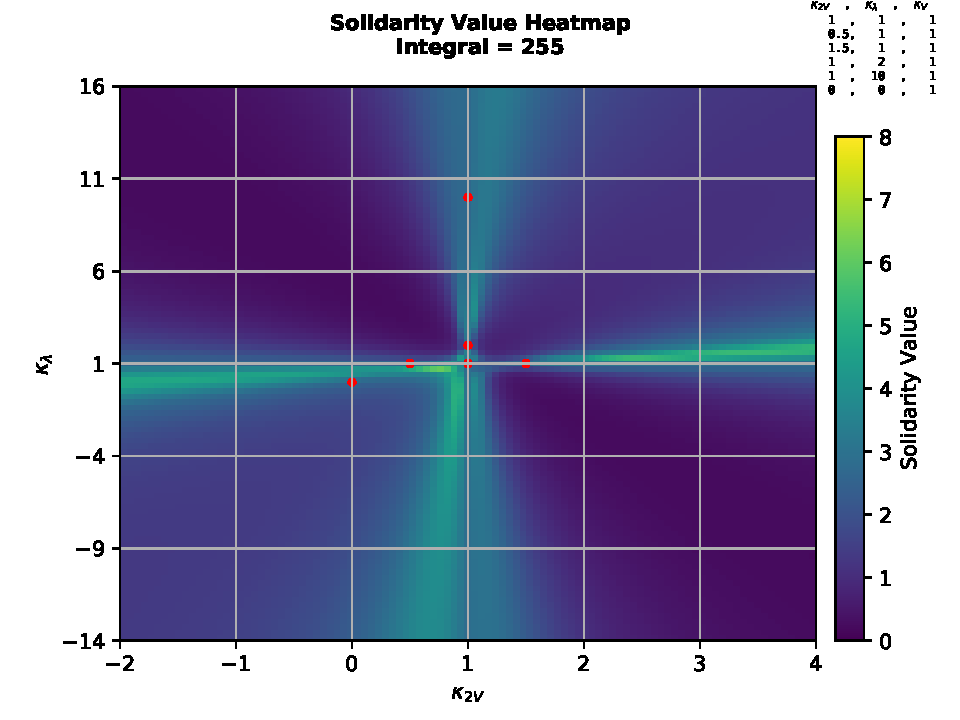
\includegraphics[width=\linewidth,height=\textheight,keepaspectratio]{signal/solidarity_main_rank00old}
            \captionsetup{justification=centering} \caption{}
        \end{subfigure}
        \begin{subfigure}{0.48\textwidth}
            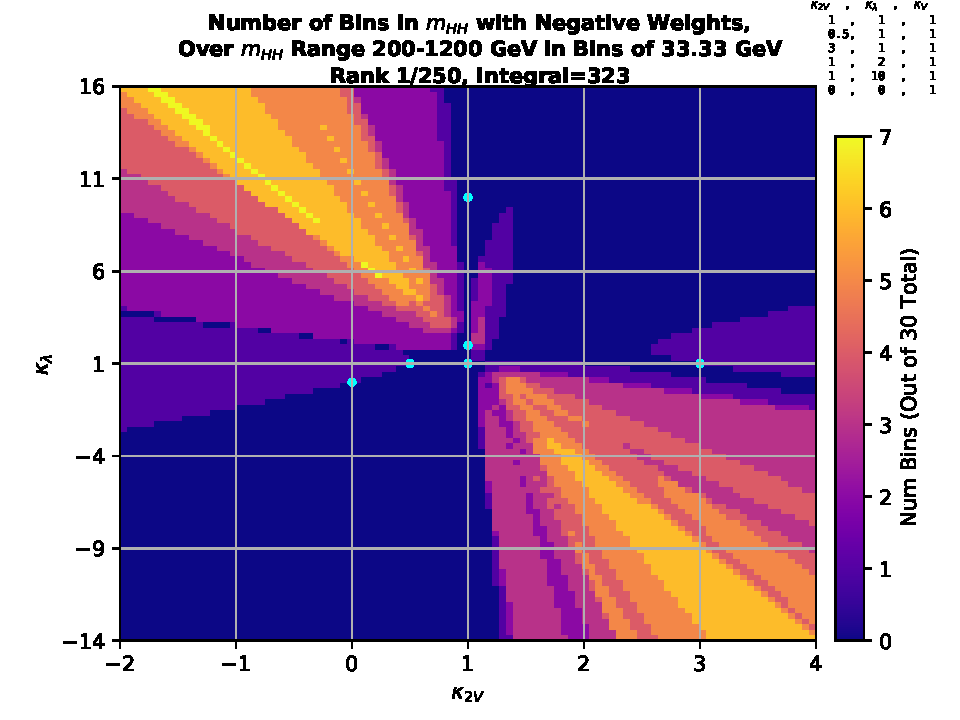
\includegraphics[width=\linewidth,height=\textheight,keepaspectratio]{signal/negative_weights_toprank0}
            \captionsetup{justification=centering} \caption{}
        \end{subfigure}
        \\
        \begin{subfigure}{0.48\textwidth}
            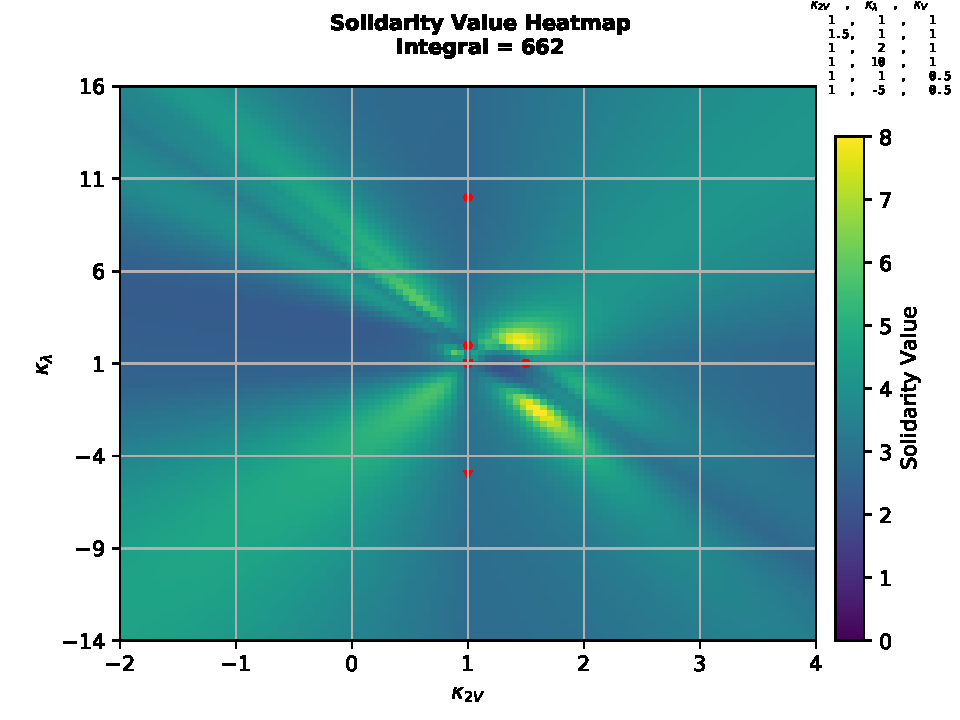
\includegraphics[width=\linewidth,height=\textheight,keepaspectratio]{signal/solidarity_main_rank01}
            \captionsetup{justification=centering} \caption{}
        \end{subfigure}
        \begin{subfigure}{0.5\textwidth}
            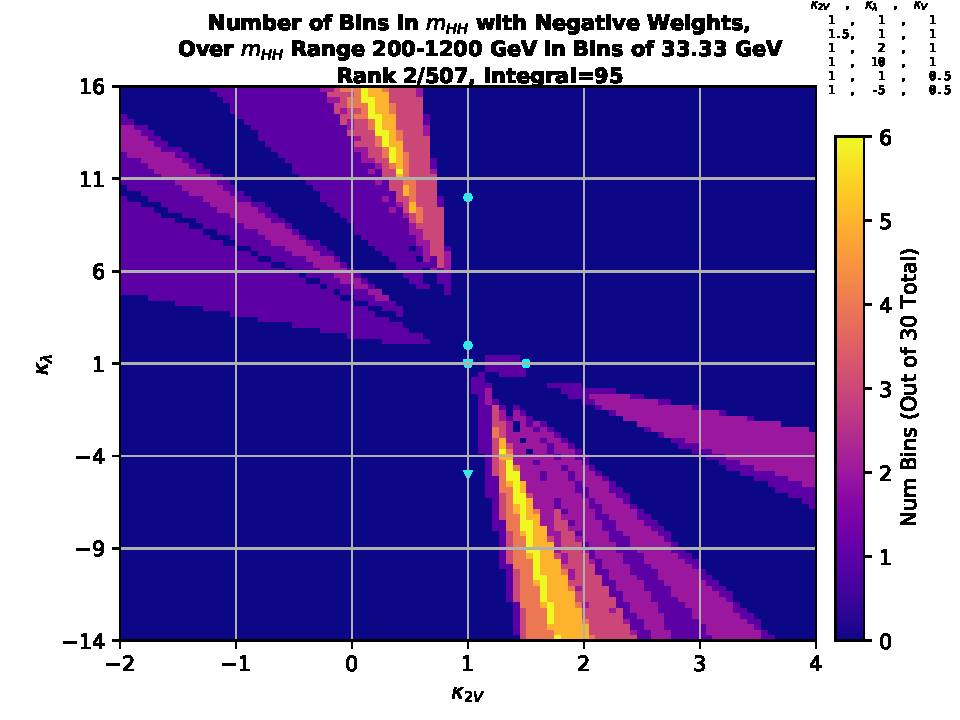
\includegraphics[width=\linewidth,height=\textheight,keepaspectratio]{signal/negative_weights_base}
            \captionsetup{justification=centering} \caption{}
        \end{subfigure}
        \caption{
            The heatmap of Solidarity calculated with theoretical cross-section values (left),
                compared to the negative weight heatmap generated by the post-reconstruction and selection MC samples (right).
            The top two plots correspond to the \textit{original} optimal basis (before the inclusion of the 13th sample),
                while the bottom two correspond to the optimal basis sample used in the analysis.
            Note that the regions of low Solidarity values correspond strongly to the regions with large numbers of negative-weighted bins.
            Also note the ``Integral'' values of the different bases (shown just below their titles).
        }
        \label{fig:solidarity_heatmaps}
    \end{figure}

    The map of Solidarity (Fig. \ref{fig:solidarity_heatmaps}) shows a strong relationship with the prevalence of negative-weighted bins,
        despite the Solidarity heatmap being calculated without the use of any MC simulation samples (beyond MadGraph).
    Using the surface integral of the heatmap as was done for the negative-weight map allows a similar metric to be given to a basis as a whole.
    Comparing this theoretical Solidarity integral to the corresponding negative weight integral (Fig. \ref{fig:nWeight_solidarity_scatter})
        shows a very strong correlation between the two,
        which can be exploited to predict useful sample bases before generating any MC samples.

    \begin{figure}[tbh]
        \begin{subfigure}{0.5\textwidth}
            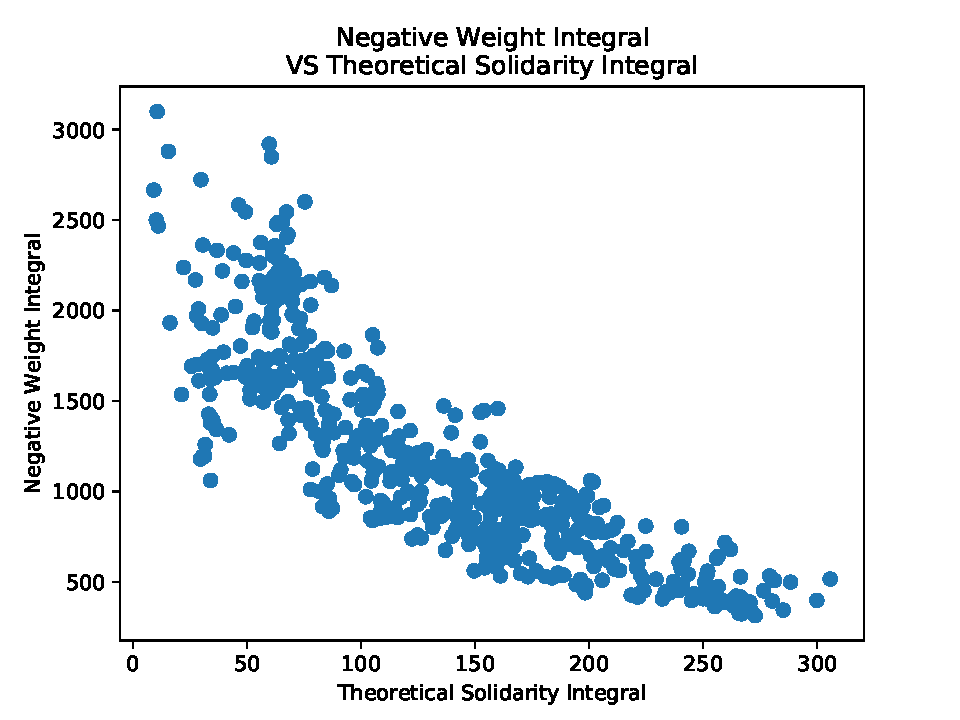
\includegraphics[width=\linewidth,height=\textheight,keepaspectratio]{signal/Nweight_integral_VS_theory_solidarity_integral_old}
            \captionsetup{justification=centering} \caption{Original 12 Samples}
        \end{subfigure}
        \begin{subfigure}{0.5\textwidth}
            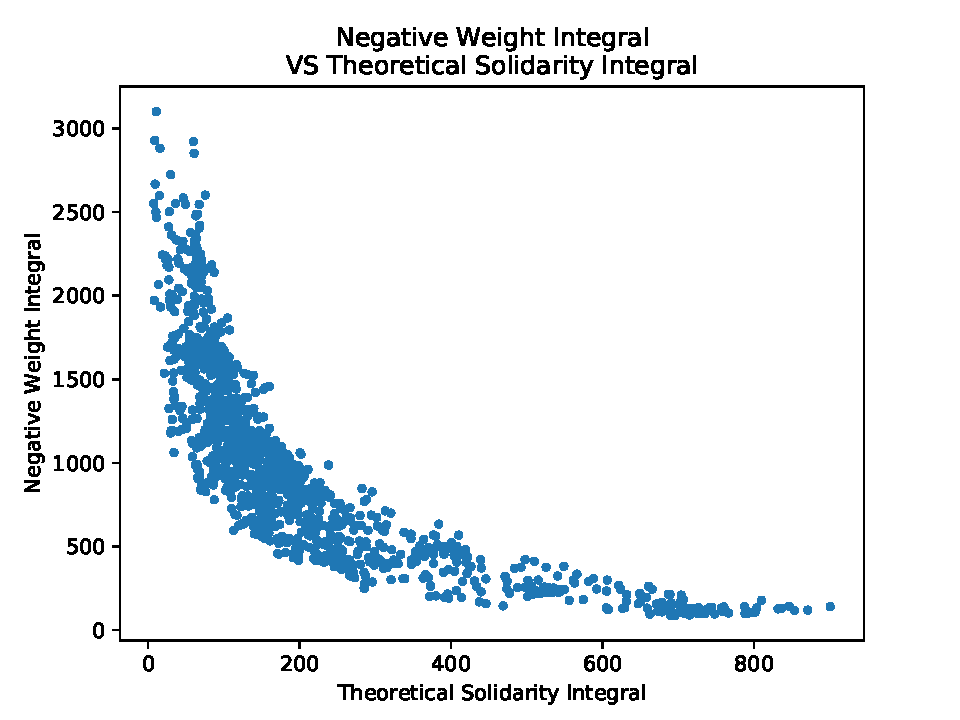
\includegraphics[width=\linewidth,height=\textheight,keepaspectratio]{signal/Nweight_integral_VS_theory_solidarity_integral}
            \captionsetup{justification=centering} \caption{Using All 13 Samples}
        \end{subfigure}
        \caption{
            Plots of the negative weight surface integral (calculated from post-reconstruction/selection MC samples)
                of all possible bases, with respect to the same bases' Solidarity surface integral
                (calculated from the theoretical cross-section associated with the MC samples' scale factor values).
            The plot on the left uses only the original 12 available MC samples for its bases.
            To the right is the same plot with the inclusion of the 13th (\kl=-5, \kvv=1, \kv=0.5) sample.
            Note that the plot on the left has a y-axis with a lower bound that is significantly higher ($\sim 250$) 
                than the full-13-sample plot (lower bound $\sim 100$),
                indicating the presence of more optimal bases afforded by the 13th sample.
        }
        \label{fig:nWeight_solidarity_scatter}
    \end{figure}


    Figure \ref{fig:nWeight_solidarity_scatter} was generated using all 1307 linearly independent bases of combining 6 of the 13 available MC samples.
    Due to the strong correlation between negative-weighted bins and solidarity,
        a histogram of only the Theoretical Solidarity surface integral
        (basically just the x-axis of Fig. \ref{fig:nWeight_solidarity_scatter})
        can be used to determine the overall potential performance a set of MC samples might have.
    In order to determine which MC sample should be produced to work most effectively with the already existing 12 samples,
        I constructed such Solidarity surface integral histograms for a wide range of possible new samples.
    Each histogram was constructed using the bases formed from all possible combinations of 6 samples from
        the 12 original samples plus one prospective MC sample.
    Thus, each Solidarity surface integral histogram corresponded to 13 samples,
        and served as a figure of merit for the 13th (the prospective) sample's performance\footnote{
            I would like to note that this brute-force application of Solidarity is far from efficient,
                and any future attempts at producing MC with this metric
                would do well to use a more sophisticated optimization technique.
        }.

    \begin{figure}[tbh]
        \begin{subfigure}{0.5\textwidth}
            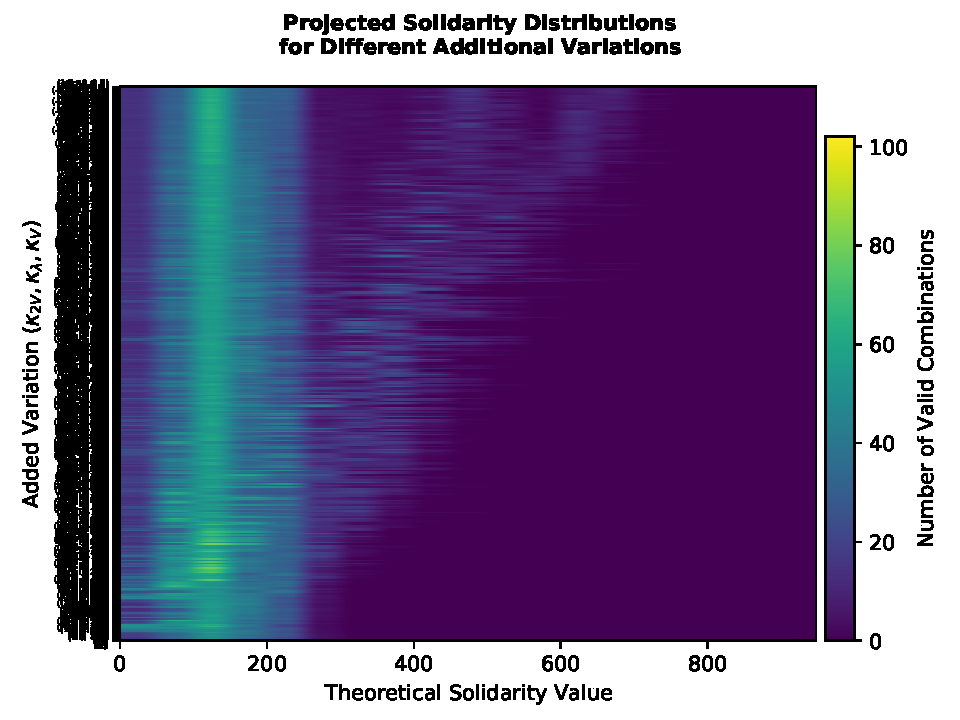
\includegraphics[width=\linewidth,height=\textheight,keepaspectratio]{signal/projective_solidarity_all}
            \captionsetup{justification=centering} \caption{All Tested ``13th'' Variation Possibilities}
        \end{subfigure}
        \begin{subfigure}{0.5\textwidth}
            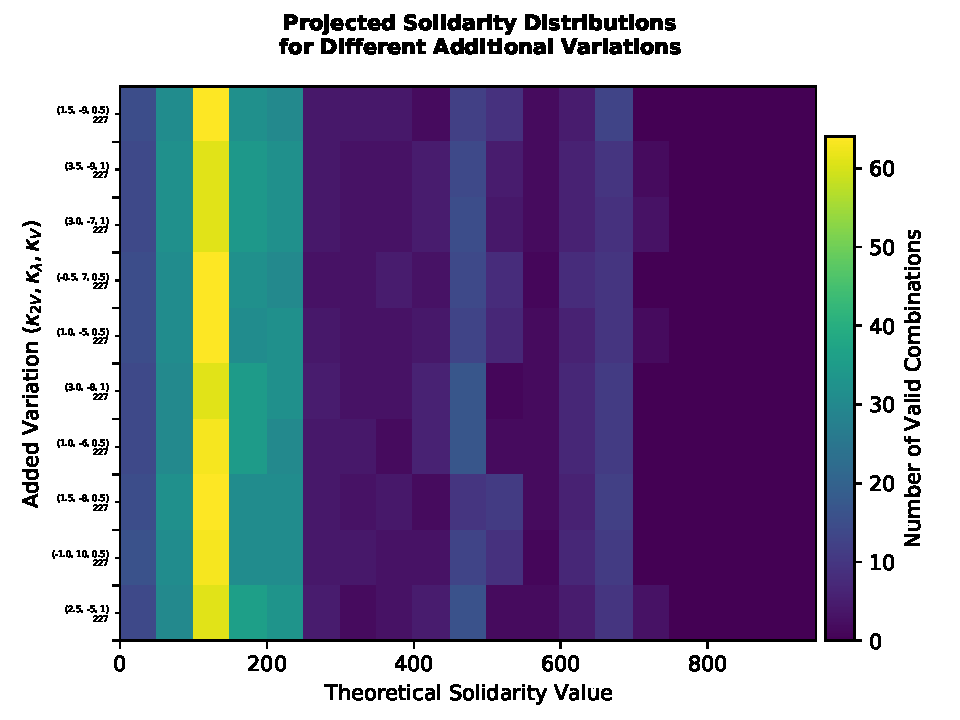
\includegraphics[width=\linewidth,height=\textheight,keepaspectratio]{signal/projective_solidarity_dump}
            \captionsetup{justification=centering} \caption{Close-up of the top of Fig. (a)}
        \end{subfigure}
        \caption{
            A 2D heatmap representation of all the Solidarity integral histograms generated for a myriad of different ``extra sample'' points.
            The rows are sorted from top to bottom by the sum of their bins
                (That is, the sum of all Solidarity surface integrals for all bases associated with the same additional MC sample point).
        }
        \label{fig:solidarity_dump}
    \end{figure}

    Aligning all of these histograms together as in Fig. \ref{fig:solidarity_dump}
        produces a clear method of distinguishing samples that 
        could produce high stability combinations with the existing 12 samples.
    The aggregate sum of all Solidarity surface integrals associated with a new sample
        can evidently be used as a scalar metric by which to rank different prospective scale factor points.
    The culmination of these tests is Fig. \ref{fig:solidarity_performance_map}.

    \begin{figure}[tbh]
        \begin{subfigure}{0.5\textwidth}
            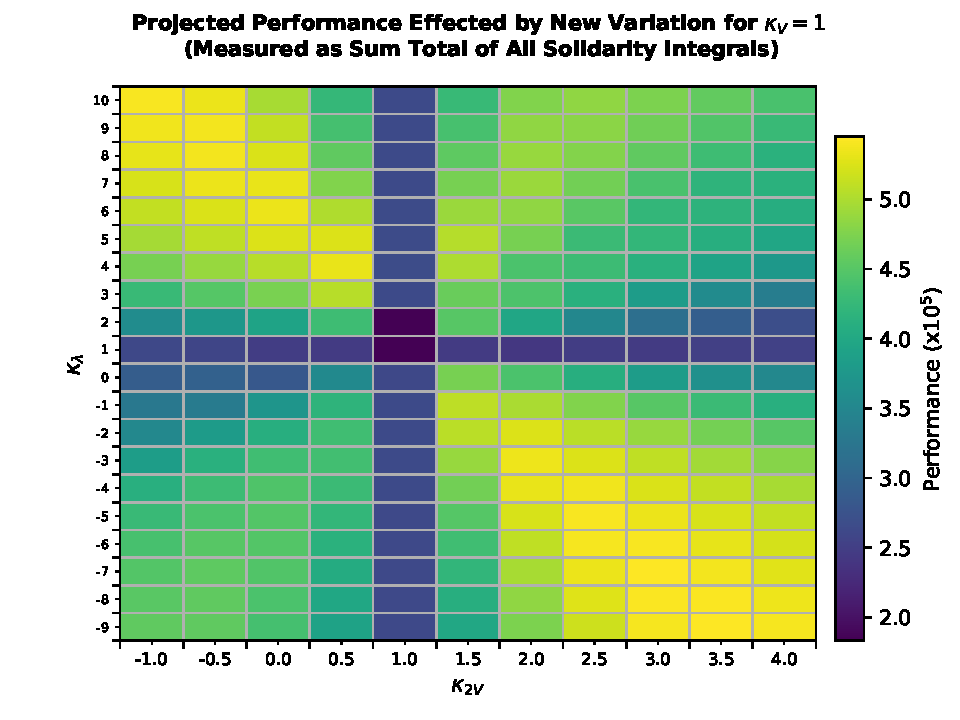
\includegraphics[width=\linewidth,height=\textheight,keepaspectratio]{signal/solidarity_performance_kv1}
            \captionsetup{justification=centering} \caption{\kv = 1}
        \end{subfigure}\\
        \begin{subfigure}{0.5\textwidth}
            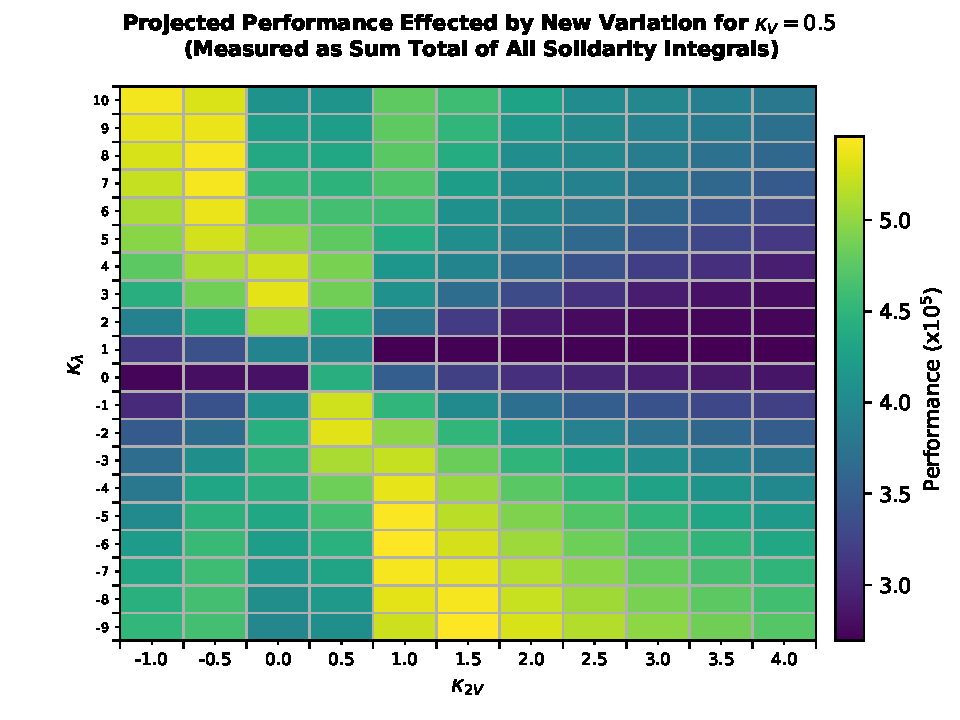
\includegraphics[width=\linewidth,height=\textheight,keepaspectratio]{signal/solidarity_performance_kv0p5.pdf}
            \captionsetup{justification=centering} \caption{\kv = 0.5}
        \end{subfigure}
        \begin{subfigure}{0.5\textwidth}
            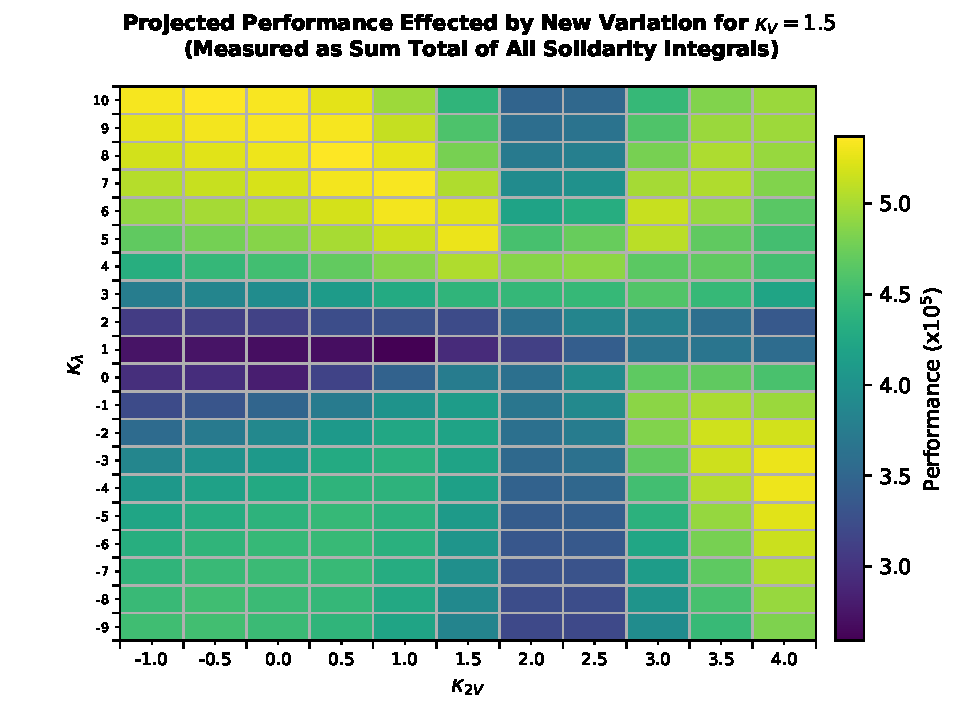
\includegraphics[width=\linewidth,height=\textheight,keepaspectratio]{signal/solidarity_performance_kv1p5.pdf}
            \captionsetup{justification=centering} \caption{\kv = 1.5}
        \end{subfigure}
        \caption{
            Solidarity cumulative performance maps for various values of \kv.
            The color of a particular (\kvv,\kl) point indicates the overall
                benefit to adding an MC sample with that set of scale factors
                to the existing set of 12 MC samples.
            Colors closer to yellow (the upper end of the scale) denote samples that would improve combination performance,
                while colors closer to purple (the lower end of the scale) denote samples that would be of little to no use if added.
        }
        \label{fig:solidarity_performance_map}
    \end{figure}

    Using Fig. \ref{fig:solidarity_performance_map} as a guide,
        a number of points (mostly those corresponding to the highest aggregate performance values, $\approx 5.5$)
        were selected for limited simulation at truth level.
    Based on the preliminary stability shown by these truth level simulations,
        a full MC production run was generated with its scale factor values set to \kvv=1, \kl=-5, \kv=0.5.
    This set of MC samples combined with the collected data and background estimation,
        can then be used together to test the validity of different possible hypotheses.

\FloatBarrier
\section{Parton Showering Uncertainty}\label{sec:sig_syst}

    Before moving onto the final results, I need to briefly address a small systematic uncertainty associated with the signal MC modelling,
        stemming from the parton showering step of simulation discussed in Section \ref{sec:pythia}.
    To account for the difficulty in accurately modelling parton showering, 
        an alternate hadronization framework, Herwig 7\cite{Bellm:2015jjp},
        is used and its output compared to Pythia8.
    Herwig performs the same function as Pythia8, but using a different technical implementation.
    The two are fairly consistent in the output kinematics they produce for the \vbfhhproc process,
        but there are slight differences (Fig. \ref{fig:pyth_herwig_mjj}).
    A systematic uncertainty is associated with this difference through the following procedure.
    First, a set of MC samples is produced through the same mechanism described in Section \ref{sec:mcsim},
        but using Herwig instead of Pythia8.
    Distributions of \mhh are formed for both of these post-selection MC samples (Fig. \ref{fig:sig_syst}),
        and a bin-by-bin difference calculated in their yields.
    This difference, normalized to the per-bin statistical error, then constitutes the systematic error.
    Now equipped with a model for the background, a model for the signal
        (for any variation of the $\kappa$-values),
        and a suitable accounting of the uncertainties associated with each,
        I can at last proceed to looking at the data and results of the analysis.

    \begin{figure}[tbh] \centering
        \includegraphics[page=64,width=\linewidth,height=0.4\textheight,keepaspectratio]{signal/V2_vbf-hh-4b_l1cvv1cv1}
        \caption{
            VBF jet invariant mass (in GeV) distribution as produced by Pythia8 and Herwig at \textit{truth-level}.
            Pythia8 is displayed in red and Herwig in blue, with their (dominating) region of overlap shown in purple.
            The differences in their behaviour are not dramatic, but are present
                (hence the relatively small associated uncertainty).
        }
        \label{fig:pyth_herwig_mjj}
    \end{figure}

    \begin{figure}
        \centering
        \begin{subfigure}{0.48\textwidth} 
            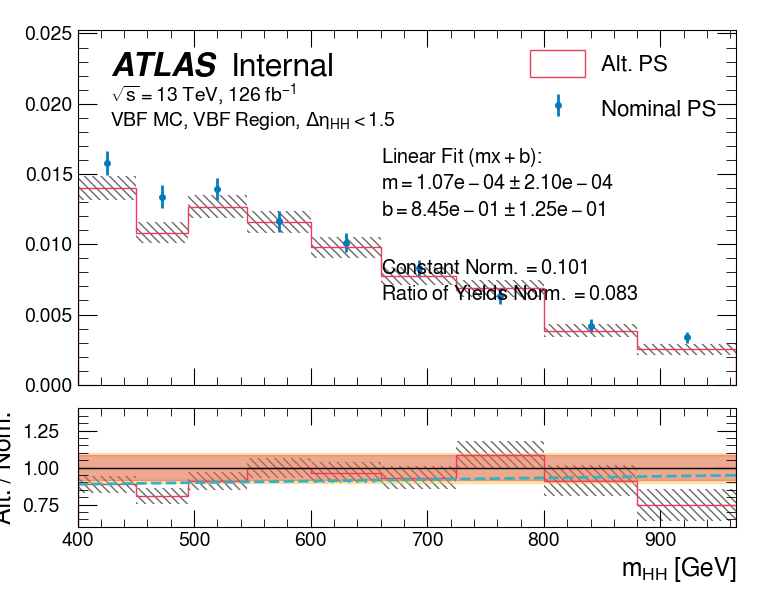
\includegraphics[width=\linewidth,height=\textheight,keepaspectratio]{signal/VBF_PS_dEta_1_20-1_kl1_k2v1}
            \caption{$\eta < 1.5$ Category}
        \end{subfigure}
        \begin{subfigure}{0.48\textwidth}
            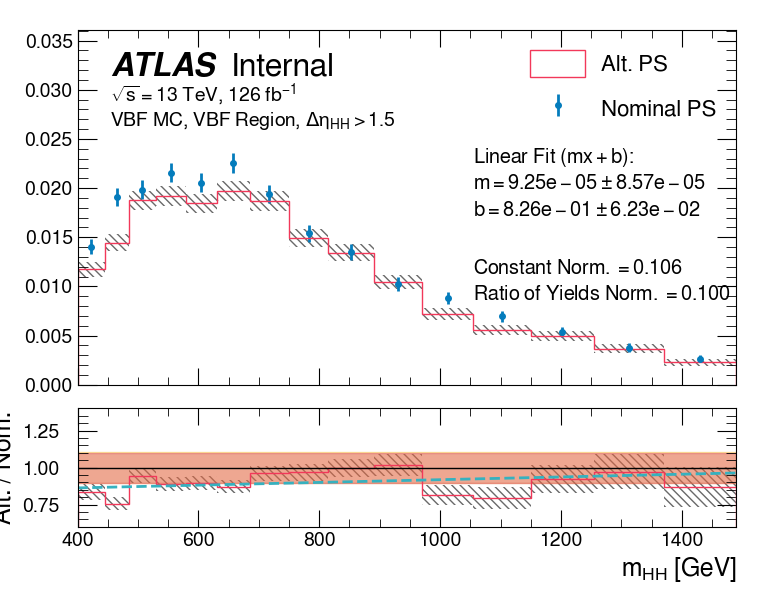
\includegraphics[width=\linewidth,height=\textheight,keepaspectratio]{signal/VBF_PS_dEta_2_20-1_kl1_k2v1}
            \caption{$\eta \geq 1.5$ Category}
        \end{subfigure}
        \caption{
            Systematic uncertainty of the parton showering step of the signal MC generation.
            The ``Nominal'' Parton Showering (PS) MC sample is that derived from Pythia8,
                while the ``Alternate'' (Alt.) sample corresponds to Herwig.
        }
        \label{fig:sig_syst}
    \end{figure}

    


%\section{I'll figure this out later I just wanna jot this down for myself first}

    Here's my more formal attempt at writing down what I do in the 2/3D interpolation

    Overall goal is to measure cross-section of an interaction: ``$\Xsec$".

    Cross-section cannot be measured directly. Instead, we must measure the total number of events ``$T$". 

    The total number of events can be related to the cross-section via the integrated luminosity $L$, by the simple relation $T = \Xsec \times L$.

    This calculation assumes that we can measure all particles across all phase space (emitted at all angles). In practice though, this is not the case.
    Many events are very forward and are never detected by the detector elements.
    Furthermore, due to the need to subtract out background events, many kinematic cuts must be placed on events, further reducing the phase space actually available.
    It is useful then to instead look at the number of events with particles existing in a particular region of phase $\mathscr{E} (q) \equiv \xsec (q) \times L$, where ``$\xsec$" is the differential cross-section.

    The total cross-section is related to the differential cross-section by the relation \\
    $\xsec (q) = d \Xsec / d q$, which can be rearanged for cross-section by integrating over phase space $q$: \\
    $\Xsec = \int \xsec (q) d q$.

    Relating this back to the event counts, we have\\
    $\frac{1}{L} T = \int \frac{1}{L} \mathscr{E} (q) dq $ \\
    $T = \int \mathscr{E} (q) dq $.

    In order to bring this in line with the fact that we cannot simulate an infinite number of events, let's decompose the integral into an infinite sum:\\
    $T = \lim\limits_{N\to\infty} \sum\limits_{n=0}^{N} \mathscr{E}(q_n) dq = \lim\limits_{N\to\infty} \sum\limits_{n=0}^{N} \mathscr{E}(q_n) \Delta q / N $.

    This total is equivalent to the theoretical value only if the number of events is infinite (and thus able to represent all of phase space).
    With a finite number of events, the theoretical total is reduced to an approximation $\tau$, where\\
    $\tau = \sum\limits_{n=0}^{N} \mathscr{E}(q_n) \Delta q / N $.

    The relative space any one event takes in phase space is accounted for in monte-carlo by giving events weights, so this can be rewritten as\\
    $\tau = \sum\limits_{n=0}^{N} w(q_n) = \sum\limits_{n=0}^{N} w_n \quad,\quad w(q_n) \equiv \mathscr{E}(q_n) \Delta q / N $.

    Final analysis of events does not count all events, but rather looks at the distribution of event counts as a function of some specific element of phase space.
    In this analysis, that element is the di-Higgs invariant mass \mhh, and so the event count per bin $m$ in \mhh can be written as\\
    $\tau_m = \sum\limits_{n=0}^{N} w_{nm} $. 

    The effects of performing reconstruction and selection can be represented by a multiplicative factor ``$z(q)$" corresponding to the probability an event with phase-space parameters $q$ will survive selection.
    What remains is the reconstructed event yield\\
    $U(q) = \int z(q) \mathscr{E}(q) dq $.

    Which can be returned to the discrete, finite-event case as\\
    $\mu = \sum\limits_{n=0}^{N} z_n * w_{nm} $.

    Note that in the infinite, continuous case, $z(q)$ is purely binary (in continuous phase-space an event either passes selection or not),
        but becomes a probability $z_n$ when regions of phase-space are aggregated together into the same bin.


\section{Sample Interpolation}

    Simulating, reconstructing, and performing selection on stuff is hard.
    We need to check all points in $\kappa$ space though.
    To address this we can exploit the underlying field-theory mechanics to reverse-engineer a general equation for the number of events expected for any value of the $\kappa$ couplings.
    First, the influence of the couplings can be related to the cross-section through the interaction amplitude ``$\amp$", where\\
    $\amp(q,\kvv,\kl,\kv) =  \kv \kl \matel_s(q) + \kv^2 \matel_t(q) + \kvv \matel_X(q) $

    The differential cross-section is just the absolute square of the amplitude,\\
    \begin{equation}\begin{split}
        \xsec(q,\kvv,\kl,\kv) = |\amp(q,\kvv,\kl,\kv)|^2 &= 
          \kv^2 \kl^2 \matel_s^2(q) + \kv^4 \matel_t^2(q) + \kvv^2 \matel_X^2(q) \\
        &+ \kv^3 \kl (\matel_s^*(q) \matel_t(q) + \matel_t^*(q) \matel_s(q)) \\
        &+ \kv \kl \kvv (\matel_s^*(q) \matel_X(q) + \matel_X^*(q) \matel_s(q) ) \\
        &+ \kv^2 \kvv (\matel_t^*(q) \matel_X(q) + \matel_X^*(q) \matel_t(q) )
    \end{split} \end{equation}

    And the abundance of matrix element cross terms can be absorbed into simple coefficients $a_i(q)$\\
    $\xsec(q,\kvv,\kl,\kv) = \kv^2 \kl^2 a_1(q) + \kv^4 a_2(q) + \kvv^2 a_3(q) + \kv^3 \kl a_4(q) + \kv \kl \kvv a_5(q) + \kv^2 \kvv a_6(q) $


    This can be further simplified by using just $\kappa$ as shorthand for all the couplings,
    so  $\xsec(q,\kvv,\kl,\kv) \to  \xsec(q,\kappa) $, and by collecting the various couplings into a vector\\
    $ \vec{f}(\kappa) = \begin{pmatrix} \kv^2 \kl^2 \\ \kv^4 \\ \kvv^2 \\ \kv^3 \kl \\ \kv \kl \kvv \\ \kv^2 \kvv \end{pmatrix} $

    So we now have\\
    $\xsec(q,\kappa) = f_1(\kappa) a_1(q) + f_2(\kappa) a_2(q) + f_3(\kappa) a_3(q) + f_4(\kappa) a_4(q) + f_5(\kappa) a_5(q) + f_6(\kappa) a_6(q) $

    Which can be written as:  
    $\xsec(q,\kappa) = \vec{a}(q) \bullet \vec{f}(\kappa) $.

    or, adopting Einstein notation, as
    $\xsec(q,\kappa) = a_i(q) f_i(\kappa) $.

    From here we can write this in terms of observed events\\ 
    $T(\kappa) = \int \xsec(q,\kappa) dq \times L = \int a_i(q) f_i(\kappa) dq \times L $.

    And in terms of post-selection events as\\
    $U(\kappa) = \int z(q) \xsec(q,\kappa) dq \times L = \int z(q) a_i(q) f_i(\kappa) dq \times L $.

    To get the number of expected events for any values of the couplings, we only need to find the reconstructed forms of $a(q)_{i}$.
    By running simulations for 6 different, linearly independent variations of $\xsec$, we can obtain the six equations needed to solve for six variables:\\
    $\xsec(q, \kappa_j) = a(q)_{i} f_i(\kappa_j) $, for $j \in {1-6}$. \\
    $\xsec(q, \kappa_j) \to  \xsec_j(q) $, $f_i(\kappa_j) \to F_{ij} $, \\
    $\xsec_{j}(q) = a(q)_{i} F_{ij}$

    Solving for $a$ is just a matter of inverting the matrix $F_{ij}$ \\
    $\xsec_{j}(q) \times F_{ij}^{-1}= a(q)_{i} F_{ij} \times F_{ij}^{-1}$ \\
    $a_{i}(q) = \xsec_{j}(q) F_{ij}^{-1}$ \\
    $a_{i}(q) = \xsec_{j}(q) G_{ji}$, with $G_{ji} \equiv F_{ij}^{-1}$ \\

    With the primed ``$\xsec'$" now denoting a linearly combined cross-section,
        the cross-section for an arbitrary value of the couplings can then be written as
    \begin{equation} \begin{split}
        \xsec'(q, \kappa) &= a_i(q) f_i(\kappa) \\
        \xsec'(q, \kappa) &= \xsec_{j}(q) G_{ji} f_i(\kappa) \\
        \xsec'(q, \kappa) &=  G_{ji} f_i(\kappa) \xsec_{j}(q) \\
        \xsec'(q, \kappa) &=  g_j(\kappa) \xsec_{j}(q) \quad, g_j(\kappa) \equiv G_{ji} f_i(\kappa)
    \end{split} \end{equation}

    Rewriting this in terms of events:
    \begin{equation} \begin{split}
        T'(\kappa) &= \int \xsec'(q,\kappa) dq \times L \\
        T'(\kappa) &= \boxed{\int g_j(\kappa) \xsec_{j}(q) dq \times L = g_j(\kappa) \int \xsec_{j}(q) dq \times L} \\
        T'(\kappa) &= g_j(\kappa) \Xsec_j \times L = g_j(\kappa) T_j \\
        T'(\kappa) &= g_j(\kappa) T_j
    \end{split} \end{equation}

    Note: the boxed section is the key to why this whole combination system works at the event-level as we use it.
    The core reason this can be done is that the $g_j(\kappa)$ coefficient
        \textit{is independant of phase space},
        and thus can be pulled out of the phase space integral.


    This can be repeated for post-selection phase-space:
    \begin{equation} \begin{split}
        U'(\kappa) &= \int z(q) \xsec'(q,\kappa) dq \times L = \int z(q) g_j(\kappa) \xsec_{j}(q) dq \times L \\
        U'(\kappa) &= g_j(\kappa) \int z(q) \xsec_{j}(q) dq \times L = g_j(\kappa) U_j
    \end{split} \end{equation}

    And performed approximately for the discrete, finite case:
    \begin{equation} \begin{split}
        U'(\kappa) &= g_j(\kappa) \int z(q) \xsec_{j}(q) dq \times L \\
        U'(\kappa) &= g_j(\kappa) \lim\limits_{N\to\infty} \sum\limits_{n=0}^{N} z(q) \xsec_{j}(q) dq \times L \\
        U'(\kappa) &= g_j(\kappa) \lim\limits_{N\to\infty} \sum\limits_{n=0}^{N} z(q_n) \xsec_{j}(q_n) \Delta q_n / N \times L \\
        U'(\kappa) \approx \mu' &= g_j(\kappa) \sum\limits_{n=0}^{N} z_n \xsec_{j,n} \Delta q_n / N \times L \\
        \mu' &= g_j(\kappa) \sum\limits_{n=0}^{N} z_n w_{j,n} \times L \\
        \mu' &= g_j(\kappa) \mu_j
    \end{split} \end{equation}



    %Since an observed event count is a collection of many individual events, this can be re-written in terms of individual event weights:\\
    %$T_m(\kappa) = G_{ji} f_i(\kappa) T_{mj}$,\\
    %$T_m(\kappa) = G_{ji} f_i(\kappa) z_{mj} \sum\limits_{n=0}^{N} w_{nmj} $. FIXME I'm not so sure about this way of describing reco-level events








